% ============================================================================
%  MSc Robotics and Computation — summer project report
%
%  Structure scaffold only. The prose is deliberately NOT written: the module
%  guidance (COMP0247 §5.5) is explicit that AI-drafted reports read shallow and
%  repetitive and mark poorly, and that any AI assistance must be credited. What
%  is here is the skeleton, the page budget, and notes on what each section has
%  to establish — the argument and the words should be yours.
%
%  One-column report class rather than a two-column article format, because the
%  results tables are wide (4-6 policy arms x TSR/collision/CI/ETS), there is
%  real display math, and the 30-page cap applies either way.
%
%  Limits (COMP0247 §5): 30 pages main body, 60 pages including bibliography and
%  appendices. Readable text size, reasonable margins, numbered pages.
% ============================================================================
\documentclass[a4paper,11pt]{report}

\usepackage[a4paper, margin=3cm, bottom=2.5cm]{geometry}
\usepackage{setspace}
\usepackage[T1]{fontenc}
\usepackage[utf8]{inputenc}
\usepackage{booktabs}      % \toprule/\midrule/\bottomrule — never use \hline
\usepackage{threeparttable} % table notes tied to the table body
\usepackage{multirow}


% --- maths -----------------------------------------------------------------
\usepackage{amsmath,amssymb,amsfonts,bm}

% --- figures and tables ----------------------------------------------------
\usepackage{graphicx}
\usepackage{booktabs}      % \toprule/\midrule/\bottomrule — never use \hline
\usepackage{siunitx}       % align numbers on the decimal point in results tables
\usepackage{subcaption}
\usepackage{multirow}
\graphicspath{{figures/}}

% --- references ------------------------------------------------------------
\usepackage[numbers,sort&compress]{natbib}   % \citet{x} -> "Author et al. [1]"
\usepackage[hidelinks]{hyperref}
\usepackage[capitalise,noabbrev]{cleveref}   % \cref{fig:x} -> "Figure 3.2"

% siunitx setup for percentage-with-CI columns
\sisetup{detect-weight=true, detect-inline-weight=math}

\newcommand{\pizero}{$\pi_{0.5}$}
\newcommand{\car}{\textsc{car}}
\newcommand{\tsr}{\textsc{tsr}}
\newcommand{\ets}{\textsc{ets}}

% ============================================================================
\title{{\vspace{-14em}
\includegraphics[scale=0.4]{ucl_logo.png}}\\
  {\Huge Project Title}\\
  {\large Optional Subtitle}\\}
\date{Submission date: Day Month Year}
\author{Candidate number: \#\#\#\#\#   % candidate number, NOT your name
  \thanks{{\bf Disclaimer:} This report is submitted as part requirement for the
    MSc Robotics and Computation at UCL. It is substantially the result of my own
    work except where explicitly indicated in the text.
    % KEEP ONLY ONE of the two disclaimers below.
    The report may be freely copied and distributed provided the source is
    explicitly acknowledged.}
  \\ \\ MSc Robotics and Computation \\ \\ Supervisor: NAME}

\begin{document}
\onehalfspacing
\maketitle

\begin{abstract}
Vision-language-action (VLA) models generalise across manipulation tasks but carry no
notion of physical safety: on the SafeLIBERO benchmark, $\pi_{0.5}$ displaces a
non-target obstacle in 82.5\% of episodes. The standard remedy is a runtime
control-barrier-function shield, which projects each proposed action onto a safe set.
It works, but it is permanent --- consuming inference budget at every control step,
requiring obstacle geometry at deployment, and adding a component that can itself fail.

This thesis asks whether that corrective behaviour can instead be amortised into the
policy's weights. Distilling $\pi_{0.5}$ on its own shielded rollouts reduced collisions
to 19.2\% \emph{with no shield at inference}, while raising task success from 58.3\% to
82.5\% on held-out initial states. One distillation round recovers most of the shielded
baseline's collision avoidance (80.8\% against 86.7\%), and the shield finds materially
less to correct when reattached, firing on 18\% of control steps against 36\%.

The transfer is bounded, and the bound is the contribution. A geometry-privileged motion
planner, safe by construction, produced no measurable improvement under a matched
comparison; filtering for successful episodes alone produced none either. What transfers
is correction at states the policy itself reaches. Four alternative mechanisms ---
scalar-reward reinforcement learning, CBF-guided sampling, language-specified safety and
best-of-$N$ selection --- were tested and rejected, each for an identified reason.
\end{abstract}


\tableofcontents
\setcounter{page}{1}

% ============================================================================
\chapter{Introduction}\label{ch:intro}
% BUDGET ~3 pages.
% Establish, in order:
%  - VLAs can follow instructions but have no notion of collision safety.
%  - Why an external safety filter is the standard answer, and why that is
%    unsatisfying: it is always needed, and it costs task success.
%  - The question this project actually asks: can the safety be moved INTO the
%    policy so the filter becomes redundant?
%  - Scope: SafeLIBERO, pi_0.5, simulation only. Say what is NOT in scope.
%  - Contributions, as a short list. Be honest about which are negative results.


\section{Motivation}

VLA models represent a paradigm shift in robotics, serving as a primary driver toward general-purpose embodied intelligence. By extending the capabilities of Vision-Language Models (VLMs) into physical execution, VLAs unify multimodal perception and low-level control into single end-to-end architectures, replacing classical modular pipelines. Pretrained on web-scale datasets and heterogeneous cross-embodiment demonstrations, these models exhibit remarkable semantic zero-shot generalization to novel objects, unseen environments, and unscripted multi-step spatial tasks.

However, deploying VLA policies into real-world, human-centric environments introduces severe safety risks. While hallucinations in pure language models merely yield incorrect text, ungrounded actions or spatial errors in VLAs directly cause physical collisions, property damage, or catastrophic injury. Unlike classical control-theoretic frameworks, neural VLA policies are uninterpretable black-box systems lacking deterministic execution bounds and safety guarantees.

Furthermore, current VLAs are highly susceptible to out-of-distribution (OOD) shifts, which trigger severe policy degradation. In long-horizon execution loops, minor perceptual or kinodynamic errors compound exponentially, causing gross trajectory drift. While external safety filters or control barrier functions can mitigate some runtime errors, they do not offer a complete solution; as shown in this work, external filtering introduces distribution shifts that can cause execution deadlocks and policy collapse. Crucially, VLAs lack intrinsic uncertainty calibration: internal policy confidence metrics do not correlate reliably with physical collision risks, rendering the model incapable of self-assessing impending failure.

\section{Problem Statement and Scope}

An unsafe VLA policy can be constrained at runtime using Control Barrier Functions (CBFs) that project unsafe nominal actions into a safe action set via Quadratic Programming (QP). On the \texttt{SafeLIBERO} benchmark, pairing the base policy ($\pi_{0.5}$) with a CBF filter drastically reduced collision rates from $82.5\%$ to $13.3\%$.

However, active runtime shielding imposes significant operational overhead:
\begin{enumerate}
    \item \textbf{Computational Overhead:} The filter must run at every control step, consuming valuable inference latency budgets.
    \item \textbf{Perceptual Dependency:} The system requires perfect, ground-truth obstacle geometry at runtime.
    \item \textbf{System Complexity:} The safety shield represents an additional single point of failure.
    \item \textbf{Policy Interactions:} Applying external CBFs post-distillation yields diminishing returns and performance degradation.
\end{enumerate}

Thus, while runtime filtering increases operational safety, it does not make the underlying policy intrinsically safe.

\paragraph{Hypothesis}
This thesis investigates whether the safe action space induced by a runtime CBF filter can be amortized directly into the parameters of a VLA policy via self-distillation. By distilling shielded rollouts back into model parameters, physical safety becomes an intrinsic property of the network rather than a runtime dependency. Beyond establishing this positive result, this work formalizes the exact boundary conditions under which such safety transfer occurs.

\paragraph{Scope and Limitations}
The empirical claims of this work are bounded by four key constraints:
\begin{itemize}
    \item \textbf{Environment:} All experiments were conducted in the \texttt{SafeLIBERO} simulated tabletop manipulation benchmark. No physical hardware experiments were performed, and no claims regarding sim-to-real transfer are asserted.
    \item \textbf{Architecture:} Model evaluations are restricted to $\pi_{0.5}$, a VLA architecture utilizing a flow-matching continuous action head. Findings related to action chunking and denoising-time interventions are specific to this model family.
    \item \textbf{Perceptual Priors:} The CBF barrier relies on privileged, ground-truth simulator geometry and scene annotations. The collision rates reported herein represent an upper bound for this class of filter, as real-world perception pipelines introduce additional estimation noise.
    \item \textbf{Statistical Bounds:} Reported statistics reflect single training runs across held-out initial states ($n = 120$ evaluation rollouts per policy configuration) evaluated at $95\%$ confidence intervals.
\end{itemize}

\section{Contributions}

The primary contributions of this work are as follows:

\begin{enumerate}
    \item \textbf{Internalization of Physical Safety via Self-Distillation:} We demonstrate that runtime safety constraints can be amortized directly into VLA weights. Without any active shield at inference time, the distilled policy reduced collision rates from $82.5\%$ to $19.2\%$ while increasing task success from $58.3\%$ to $82.5\%$ on held-out initializations. The distilled policy recovers the majority of the teacher's safety performance (Collision Avoidance Rate of $80.8\%$ vs.\ $86.7\%$) in a single behavioral cloning iteration without deployment latency.
    
    \item \textbf{Demarcation of Demonstration Sources:} We establish that safety transfer depends strictly on supervising the policy's own error distribution. Distillation using rollouts from a privileged RRT motion planner failed completely; the resulting student was statistically indistinguishable from the baseline. Effective transfer requires correcting the model's own execution failures rather than exposing it to external expert trajectories.
    
    \item \textbf{Disambiguation of Correction vs. Success Filtering:} Through matched N=85 control experiments, we prove that safety gains stem from active step-wise CBF corrections during rollout generation rather than outcome-based success filtering alone ($84.2\%$ vs.\ $26.7\%$ success, with disjoint confidence intervals).
    
    \item \textbf{Dual-Channel Safety Transfer:} We discover that safety transfers through two distinct mechanisms:
    \begin{itemize}
        \item \emph{Direct Correction Imitation:} Where the CBF is precise (end-effector boundaries), the student learns directly from the filter's corrections.
        \item \emph{Outcome Selection on Imperfect Signals:} The CBF shield eliminated end-effector collisions completely ($71 \to 0$ across $360$ episodes) but permitted $15$ arm-link collisions. Remarkably, the unshielded distilled student achieved only $8$ arm-link collisions—outperforming its own teacher. This occurs because trajectory retention criteria filtered out all link contacts, allowing the student to learn full-body spatial avoidance beyond what the analytical shield explicitly enforced.
    \end{itemize}
    
    \item \textbf{Empirical Analysis of Alternative Adaptation Schemes:} We systematically evaluate and reject four alternative adaptation mechanisms—scalar-reward reinforcement learning, CBF-guided sampling, language-conditioned safety prompting, and best-of-$N$ sample selection—providing mechanistic explanations for why each fails to enforce low-level physical invariance.
\end{enumerate}
% ============================================================================
\chapter{Background and Related Work}\label{ch:background}

\section{VLA Models and the Safety Problem They Inherit}
\label{sec:bg:vla}

VLA models map camera observations and a natural-language instruction
directly to continuous robot actions, and have become the dominant paradigm for general-purpose
manipulation. The policy studied here, $\pi_{0.5}$, pairs a pretrained VLM backbone
with a flow-matching action expert that emits chunks of continuous actions, and is trained by
heterogeneous co-training across robot demonstrations, semantic subtask prediction, and
web-derived multimodal data~\cite{physicalintelligence2025pi05}. The flow-matching action expert
is inherited from its predecessor~\cite{black2024pi0}.

What matters for this thesis is what that training does \emph{not} optimise. These models are
built and evaluated for generalization ability as the main goa. Nothing in the objective penalises contact with an
object that is not the target, and the collected dataset doesn't prioritize near-collision or collision avoidance settings. Task
competence is not evidence of physical safety, and no collision-safety claim is made in
the work introducing the model~\cite{physicalintelligence2025pi05}.

The base policy collides in more than eight of every ten episodes of the SafeLIBERO benchmark (Section~\ref{sec:shield_efficacy}). The problem address here therefore is that competence and safety are separate properties, and only the former has been optimised.

\section{Control Barrier Functions}\label{sec:bg:cbf}

Control theory offers a mature answer to constraint satisfaction. A CBF
encodes a safe set $\mathcal{C}$ as the superlevel set of a differentiable function $h$, and
converts safety into a condition that is affine in the control input: any $u$ satisfying
$\dot{h}(x,u) \ge -\alpha(h(x))$ renders $\mathcal{C}$ forward invariant, so a system that begins
safe remains safe~\cite{ames2017cbf}.

Because the condition is affine in $u$, it can be imposed as one linear inequality per constraint
inside a quadratic program that stays as close as possible to a nominal input,
\begin{equation}
  u^{\star} = \arg\min_{u} \tfrac{1}{2}\lVert u - u_{\mathrm{nom}} \rVert^{2}
  \quad \text{s.t.} \quad
  \nabla h^{\top}\!\left(f + gu\right) \ge -\alpha(h).
  \label{eq:cbf_qp}
\end{equation}
This is the object the rest of the thesis calls a \emph{shield}: a filter that accepts whatever a
nominal controller proposes and returns the minimum modification satisfying the constraint. Two
properties make it attractive as a teacher rather than merely as a guard. It is agnostic to how the
nominal action was produced, so it composes with a policy it knows nothing about; and its output is
\emph{the closest safe action to the policy's original output}, which is the optimal form for a supervised
learning target.

Two caveats bound what may be claimed later. The guarantee is continuous-time and assumes known
control-affine dynamics, so a discrete-time implementation on a contact-rich manipulator satisfies
it only approximately (Section~\ref{sec:shield}). And forward invariance is a property of the
\emph{closed loop containing the quadratic program}. Removing the program also removes the guarantee;
Section~\ref{sec:bg:learned} returns to how much of it can be recovered.

\section{Runtime Shielding for VLA Models}\label{sec:bg:shielding}

The immediate prior work applies this machinery to VLAs directly. AEGIS mounts a safety layer on $\pi_{0.5}$: a vision--language module extracts obstacle geometry, and a CBF-QP modifies the policy's proposed action whenever it
violates the resulting constraint. That work also contributes SafeLIBERO, the benchmark used
here~\cite{vlsa2026}, which augments the LIBERO manipulation suite~\cite{liu2023libero} with obstacles at two difficulty levels.

The approach works, and this thesis reproduces its unshielded baseline closely --- collision
avoidance of 17.5\% against their 17.3\%, task success 58.3\% against 58.9\%, on the three suites
used here (Section~\ref{sec:shield_efficacy}).

Two limitations of that work motivate the approaches explored in this work. Firstly, the layer is a
\emph{permanent}external fixture: it runs a QP at every control step, requires obstacle geometry at
deployment, and adds a component that can itself fail. 

The second is a limitation stated by the authors themselves, and is measured directly in this work.
Enforcing safety at inference can push the policy into out-of-distribution states, where the
policy may behave erratically and fail to recover --- an effect they name \emph{safety-induced
distribution shift}~\cite{vlsa2026}. Section~\ref{sec:res:internalise} measures this as a
success cost of shielding, and it is a strong argument that a permanent filter is not the ultimate
goal.

One further methodological difference is worth mentioning. The AEGIS's formulation solely constrains the end-effector, and consequently unconstrained kinematic links may collide~\cite{vlsa2026}. The barrier built in
Section~\ref{sec:barrier} additionally constrains the wrist and links three through seven, an
extension whose consequences Section~\ref{sec:res:scope} quantifies.

\section{Learned Safety Representations, and Why They Still Optimise at Deployment}
\label{sec:bg:learned}

A parallel approach removes the need for an analytically specified barrier by learning
one. ConBaT trains a causal transformer with a safety critic from binary safe/unsafe labels, and operates in embedding space rather than state space so
it applies where geometry is unavailable~\cite{meng2024conbat}. Latent Policy Barrier treats the
latent manifold of expert demonstrations as an implicit barrier, training a dynamics model on both
expert data and the policy's own rollouts, then detecting and correcting departures from that
manifold~\cite{sun2025lpb}.

Latent Policy Barrier is the closer of the two to this thesis, because its recovery data comes from
the policy's own rollout distribution --- checkpoints saved during training, executed to gather
deviations without requiring success labels, task rewards or human teleoperation.

But both retain the property that motivated this work. ConBaT performs lightweight online
optimisation at deployment, rectifying actions by backpropagation through its critic until the CBF
conditions hold~\cite{meng2024conbat}. Latent Policy Barrier performs inference-time steering in
latent space, running gradient-based corrections through its dynamics model at every step, and
explicitly advertises plug-and-play compatibility with off-the-shelf pretrained policies without
requiring retraining or fine-tuning~\cite{sun2025lpb}. Their goal is the inverse of the one here:
they improve a frozen policy by adding machinery, where this thesis improves the policy so the
machinery can be discarded.

This motivates the question of how much safety can transferred to the weights.Cosner et al.\ establish conditions under which imitating a CBF-based expert yields a learned controller with safety guarantees~\cite{cosner2022il_cbf}. The result is genuine but
demanding: the expert must be a \emph{robust} CBF-QP with explicit disturbance margins, dynamics must be known and control-affine, and the learned controller must satisfy a
CBF-compliancy condition requiring data density along the safe-set boundary, bounded learning
error, and a known Lipschitz constant --- and even then the guarantee holds on an \emph{expanded}
safe set that degrades with data sparsity and learning error.

None of those conditions is met here, and Section~\ref{sec:disc:limitations} documents which and why. Nonetheless, their Remark 1 is a core motivator of this work's approach: the goal is to transfer safety guarantees from the expert controller to the learned controller rather than just mimicking the expert's behaviour~\cite{cosner2022il_cbf}. Safety transfer is not imitation
fidelity --- a distinction Section~\ref{sec:res:scope} observes empirically, where the distilled
policy avoids arm-link collisions better than its teacher.

\section{What Makes Corrective Data Transfer}\label{sec:bg:corrective}

The central question of this thesis is not whether a policy can be trained on corrected actions,
but which corrections teach. Three approaches converge on an answer, and together they supply
the hypothesis that Chapter~\ref{ch:results} tests.

SAFE-GIL injects reachability-computed adversarial disturbances during data collection, steering a
fixed expert toward the states a learner's errors would produce so that its recovery behaviour is
recorded~\cite{ciftci2025safegil}. Their ablation is decisive: Gaussian noise, uniform
noise and DART all fail to reproduce the safety benefit, so the \emph{targeting} of the disturbance, not augmentation, is what matters. IntervenGen reaches a similar conclusion, rolling out the current policy so that recorded mistakes are its own,
then transforming human recovery segments onto the states reached~\cite{hoque2024intervengen};
they report that ten interventions expanded synthetically outperform a hundred collected directly.

In SAFE-GIL the expert is an MPC or PID controller; in IntervenGen the recovery actions come from a human
teleoperator. Neither teacher is the learner, and in both cases safety transfers. What the
two share is not the identity of the teacher but the location of the supervision: corrections are
supplied at states the learner itself would reach. The hypothesis this thesis inherits from them is
therefore about state coverage, and Section~\ref{sec:res:source}'s planner comparison is a test of
it rather than a demonstration that foreign controllers cannot teach.

ROAD-VLA constructs a proximal teacher by perturbing the student's own action-token logits with calibrated advantage estimates, and distils that teacher along the student's on-policy rollouts, with a policy-improvement bound that holds only while the teacher remains close to the current policy~\cite{wang2026roadvla}. Every variant it rejects is \emph{textual} and the teacher it accepts is derived from the student itself, so no foreign low-level controller is tested in that work.

Finally, one result establishes that the protocol used here is not sufficient on its own. Guerrier
et al.\ train a RL agent with a CBF filter active throughout training and then
remove it~\cite{guerrier2025guardrails}. Safety is not retained: the agent collides once the filter
is disabled, and their critic assigns high value \emph{inside} the obstacle. Their agent's actions
were overridden, but its objective remained a scalar reward, so no gradient ever pointed toward the
corrected action. Their curriculum variant, which blends filter and policy actions with the
filter's weight decayed to zero, does internalise the constraint.

That negative is what makes this thesis's question non-trivial. Being trained under a shield does
not make a policy safe; what the policy is trained \emph{on} decides the outcome.

\section{Policy-Level Safety Learning as an Alternative Route}\label{sec:bg:saferl}

Runtime filtering and corrective imitation are not the only options. SafeVLA formulates VLA safety as a constrained Markov decision process, eliciting unsafe
behaviour and optimising the policy under explicit constraints~\cite{safevla}. SafeDojo performs
model-based safe RL inside an action-conditioned video world model, estimating
imagined task progress and safety cost separately and optimising them with Lagrangian constrained
GRPO --- and evaluates on SafeLIBERO, making it the most direct methodological alternative in this
literature~\cite{safedojo}.

\section{The Gap}\label{sec:bg:gap}

The literature above establishes five things. Runtime CBF shielding makes VLAs measurably safer and
is the state of the art for this benchmark, at the cost of a permanent inference-time component and
a distribution shift~\cite{vlsa2026}. Learned barriers relax the need for
analytic constraints but continue to optimise at
deployment~\cite{meng2024conbat,sun2025lpb}. Imitation of a CBF-safe expert can in principle
transfer formal guarantees, under conditions no large visuomotor policy currently
satisfies~\cite{cosner2022il_cbf}. Corrective data transfers when it covers the states the learner
reaches, irrespective of who produced
them~\cite{ciftci2025safegil,hoque2024intervengen,wang2026roadvla}. And exposure to a shield during
training does not, by itself, internalise safety~\cite{guerrier2025guardrails}.

But a question remains to be answered: whether the corrections a control-theoretic
shield produces can be compiled into a VLA's weights so that the shield can be removed, and what bounds that transfer.

What is new is the conjunction: a control-theoretic safety filter, distilled from a VLA's own shielded rollouts, evaluated with the filter removed,  --- together with the boundary condition that a geometry-privileged planner, safe by construction and supplying well-formed low-level
actions, does not transfer under a matched comparison. 


\chapter{Method}\label{ch:method}

\section{The SafeLIBERO Benchmark}\label{sec:benchmark}

All experiments use SafeLIBERO~\cite{vlsa2026}, which augments the LIBERO manipulation
suite~\cite{liu2023libero} with obstacles placed in the workspace. The grid is three
task suites (spatial, object, goal) $\times$ two obstacle levels $\times$ four tasks, giving 24
distinct scenes, each providing 50 randomised initial states.

Initial states 0--34 are used for demonstration collection and training; states 35--49 are held out
and used only for evaluation. Every result in Chapter~\ref{ch:results} evaluates five held-out
initial states per scene, giving $n = 120$ rollouts per condition. Rollouts run for a horizon of
300 control steps, with the policy queried every five steps and the next five actions of the
emitted chunk executed before the next query.

\subsection{Metrics}\label{sec:metrics}

\paragraph{Task success rate (TSR)} is the fraction of rollouts in which the environment's own goal
predicate is satisfied at any point before the
horizon expires. Success is binary per rollout.

\paragraph{Collision} is recorded when the obstacle's position departs from its initial position by more than one millimetre in the $\ell_1$ sense,
\begin{equation}
  \sum_{k \in \{x,y,z\}} \bigl| p_k(t) - p_k(0) \bigr| > 0.001~\mathrm{m},
  \label{eq:collision}
\end{equation}
and a rollout is marked collided if this holds at any control step. Collision-avoidance rate (CAR) is the complement.

\paragraph{Execution time to success (ETS)} is the control step at which the success predicate
first holds, averaged over successful rollouts only and reported in control steps. ETS is therefore conditional on success and must be read
alongside TSR.

\paragraph{CBF activation rate} is the fraction of control steps on which the shield altered the
action, counted whenever the projected action differs from the nominal by more than $10^{-4}$ in
norm. It measures how \emph{often} the shield intervened, not how large the corrections were, and
serves as an independent check on internalisation: a policy that has learned to avoid obstacles
should need fewer corrections when the shield is reattached.

\paragraph{Mean correction norm} is the average $\lVert u^{\star} - u_{\mathrm{nom}} \rVert$ over steps where the shield intervened, measured against actions bounded to $[-1,1]$ per axis. Where the activation rate says how often the shield acted, this says how far it moved the action when it did. The two are independent: a shield could intervene constantly with negligible corrections, or rarely with large ones.

All proportions are reported with 95\% Wilson score confidence intervals.

Unless a caption states otherwise, every reported condition is $n = 120$ held-out rollouts pooled over the 24 scenes, with proportions given as Wilson 95% intervals.

\section{Obstacle Geometry and the Barrier}\label{sec:barrier}

The obstacle's collision mesh is read from the simulator, sampled into a point cloud, and decomposed
into a small set of spheres. Sphere decomposition is used rather than a single bounding volume
because a bounding sphere over a non-convex object is a poor approximation.

\paragraph{End-effector.} Three spheres in the end-effector frame approximate the Franka hand: a
palm sphere of radius 4.8\,cm at 5.6\,cm behind the grasp site, and two finger-pad spheres of
radius 2.0\,cm offset 3.6\,cm either side at 10.5\,cm depth.

\paragraph{Arm links.} Links three through seven and the palm body are each assigned a radius
(5.5\,cm to 9.0\,cm, set from the link's maximum transverse extent plus a 15--21\,mm margin) and
sampled at three positions along the link axis, so a long link is not represented by its origin
alone.

For each pair of a robot sphere $i$ and an obstacle sphere $j$ the barrier is
\begin{equation}
  h_{ij} = \lVert p_i - c_j \rVert^{2} - (r_i + r_j)^{2},
  \label{eq:barrier}
\end{equation}
with $h > 0$ the safe set. Differentiating along the rigid-body velocity gives the constraint row
\begin{equation}
  \bigl[\, 2\,s\,(p_i - c_j)^{\top} R_1 \,\bigr]\, u \;+\; k\,h_{ij} \;\ge\; 0,
  \qquad k = 10,
  \label{eq:constraint_row}
\end{equation}
where $u$ is the commanded end-effector velocity in the body frame, $R_1$ its rotation and $s$ a
scale factor. For arm links, whose velocity is not the commanded one, the mapping
$v_{\mathrm{link}} \approx J_{\mathrm{link}} J_{\mathrm{ee}}^{+}\,(s R_1 u)$ is used, with
$J_{\mathrm{ee}}^{+}$ a damped pseudo-inverse ($\lambda = 10^{-3}$).

Five properties of this construction bear on Chapter~\ref{ch:results}.

\begin{itemize}
  \item \emph{The robot model is approximate} The end-effector is covered by
  three fitted spheres; each arm link by three point samples carrying one radius. The end-effector
  is represented more faithfully than the links.

  \item \emph{Links one and two are not constrained}, being close to the base and rarely
  near the obstacle in these scenes.

  \item \emph{Arm-link velocities are estimated, not commanded.} The QP optimises an
  end-effector velocity and infers each link's motion through a damped Jacobian pseudo-inverse.
  Where that inverse is ill-conditioned, the predicted
  link velocity and the realised one diverge, and the constraint is enforced against the
  prediction.

  \item \emph{The geometry is privileged.} The barrier is constructed from ground-truth obstacle geometry taken directly from the simulator,
not from perception. A deployed system would have to estimate that geometry from sensors and would
inherit the resulting error. The numbers here should therefore be read as an upper bound on what
this class of shield achieves, with the perception gap removed by construction.

  \item \emph{Arm links are constrained here but not in the originating work}, whose formulation
  solely constrains the end-effector and which notes that its unconstrained kinematic links may
  consequently collide~\cite{vlsa2026}. Extending the barrier to the links is a deliberate
  difference from that baseline, and Section~\ref{sec:shield_efficacy} reports its effect.
\end{itemize}

\section{The CBF Shield}\label{sec:shield}

At each control step the policy's proposed translation is treated as a nominal end-effector
velocity $u_{\mathrm{nom}}$, and the shield solves
\begin{equation}
  u^{\star} = \arg\min_{u} \lVert u - u_{\mathrm{nom}} \rVert^{2}
  \quad \text{s.t.} \quad
  a_m^{\top} u + b_m \ge 0 \;\; \text{for every constraint row } m,
  \label{eq:shield_qp}
\end{equation}
a quadratic program in three variables whose rows are the end-effector/obstacle and arm-link pairs
of Section~\ref{sec:barrier}. This is the standard CBF-QP form~\cite{ames2017cbf}, instantiated on
the sphere-pair barrier of Equation~\ref{eq:barrier}. When no constraint is active the solution is $u_{\mathrm{nom}}$ and the action passes through unchanged.

\begin{figure}[htbp]
  \centering
  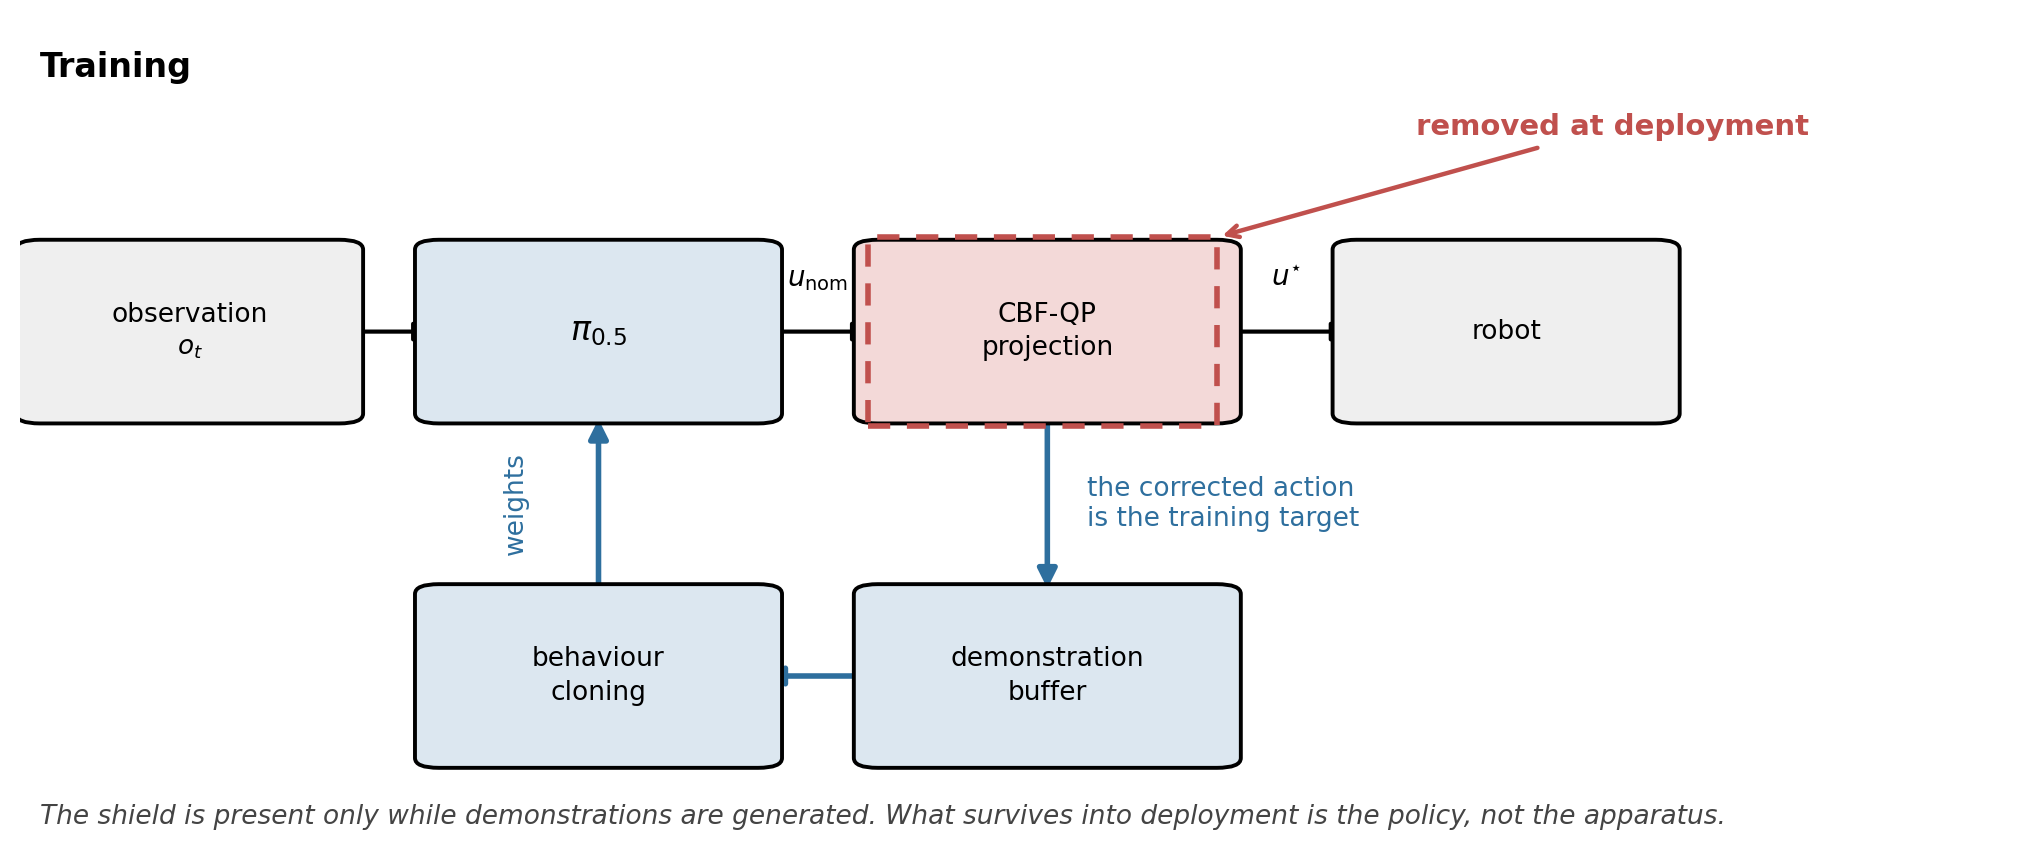
\includegraphics[width=\linewidth]{figures/fig_shield_block.png}
  \caption{Training Loop}
  \label{fig:shield_block}
\end{figure}

The problem is solved with OSQP~\cite{stellato2020osqp} through
CVXPY~\cite{diamond2016cvxpy}. An intervention is recorded when the returned action differs from the nominal by more than $10^{-4}$.

Two discrete-time adjustments are required because the barrier's guarantee is continuous-time. The
effective radius is inflated by a lag buffer covering the distance travelled between control steps
and the inverse-kinematics tracking error. Rotation is not constrained: the barrier acts
on the translational channel only.

\section{Collision Attribution}\label{sec:attribution}

Because the barrier's authority is uneven across the robot, the distinction is essential to
interpreting the residual, so each episode additionally records which bodies contacted the
obstacle, grouped as gripper, arm link, held object, and other scene objects.

\section{Teachers}\label{sec:teachers}

Two sources of demonstrations are compared, and the comparison between them is the central
experiment of this work.

\subsection{The Shielded Policy as Its Own Teacher}\label{sec:teacher_self}

The policy is rolled out with the shield active, and episodes are retained if they succeeded,
displaced nothing, and the shield intervened at least once. That third criterion matters: a clean
episode in which the shield never fired is ordinary base-policy behaviour and teaches nothing about
safety.

\subsection{A Privileged Scripted Expert}\label{sec:teacher_planner}

The alternative teacher is a sampling-based motion planner: RRT-Connect in joint space with
clearance inflation, followed by inverse kinematics and playback as operational-space deltas.
It reads object and goal poses directly from the BDDL scene specification~\cite{liu2023libero}.

The planner produces collision-free plans, but not collision-free executions: inverse-kinematics
tracking error and operational-space control cause the realised trajectory to depart from the
planned one. Its demonstrations are therefore collected under the same shield as the policy's
own (Section~\ref{sec:shield}). The two teachers differ in the states their demonstrations
occupy, not in whether they were corrected --- the planner plans from its own initial
conditions and is never conditioned on where $\pi_{0.5}$ fails.


\subsection{Why \texorpdfstring{$\pi_{0.5}$}{pi 0.5}, and What Was Tried First}
\label{sec:base_choice}

The work began on OpenVLA-7B with a Cartesian CBF filter, and the first
distillation attempt collected CBF-corrected demonstrations and fine-tuned that model through LoRA.
It produced no useful learning signal.

OpenVLA-7B's base competence on LIBERO is low enough that safety and capability failures are difficult to separate: a policy that rarely completes the task provides
little opportunity to observe whether it completes it \emph{safely}.

$\pi_{0.5}$ has substantially stronger base LIBERO
performance, which makes the safety question well-posed, and it is the policy the runtime-shielding
baseline evaluates~\cite{vlsa2026}, which makes the comparison in
Section~\ref{sec:shield_efficacy} direct.

\section{Distillation}\label{sec:distillation}

Retained demonstrations are behaviour-cloned using the model's native flow-matching
loss~\cite{physicalintelligence2025pi05,black2024pi0}. Only the parameters selected by the training
configuration's trainable filter receive gradients --- a LoRA adapter on the action head --- while
the vision-language backbone is frozen. The imitation target is the sequence of actions actually executed,
that is post-shield, so the policy learns the corrected behaviour rather than its own original
proposals. Actions are normalised by passing them through the policy's own input transform, so the
target matches the distribution the model was pretrained on rather than a hand-rolled
normalisation.

The procedure sits in the DAgger lineage~\cite{ross2011dagger}, and shares with
SafeDAgger~\cite{zhang2017safedagger} the idea that a safe controller's interventions are
themselves the informative signal. 

\paragraph{Training Control and Alignment}
When comparing distilled policies, training runs are matched strictly on the total number of gradient steps rather than the number of epochs. This controls for disparities in episode lengths across demonstration sources: a shielded VLA rollout over a horizon of 300 steps yields approximately 35 training samples, whereas a scripted motion planner episode over a 900-step horizon yields approximately 412 samples. Matching by epoch count would result in severe step imbalances ($16{,}140$ vs.\ $\approx 212{,}000$ gradient steps). The distilled policies compared are matched at $16{,}140$ and $15{,}988$ gradient steps respectively (a variance of $<1\%$).

\chapter{Experiments and Results}\label{ch:results}

\section{Experimental Setup}

\paragraph{Action Generation and Integration Dynamics}
Each action chunk is generated by integrating the velocity field of $\pi_{0.5}$. Under the linear flow transport equation:
\begin{equation}
    x_t = t \epsilon + (1 - t) a,
\end{equation}
the latent variable at $t = 1$ is a Gaussian sample $\epsilon \sim \mathcal{N}(0, \mathbf{I})$, and the latent variable at $t = 0$ corresponds to the generated action $a$. Generating an action chunk thus requires numerical integration of the learned velocity field from $t = 1$ to $t = 0$, for which ten denoising steps are used.



\section{Does the Shield Make \texorpdfstring{$\pi_{0.5}$}{pi 0.5} Safe?}\label{sec:shield_efficacy}

The first question is whether a control barrier function shield, applied as a runtime filter, makes
a pretrained VLA safe on this benchmark at all. Table~\ref{tab:shield_efficacy} reports the
comparison: the shield removes 69 percentage points of collision, with disjoint confidence
intervals.

\begin{table}[htbp]
\centering
\caption{Safety and task performance for base $\pi_{0.5}$ with and without the CBF runtime shield.
  Pooled over 24 scenes, $n = 120$ held-out rollouts per condition, Wilson 95\% intervals.}
\label{tab:shield_efficacy}
\begin{tabular}{lccc}
\toprule
\textbf{Policy} & \textbf{TSR (95\% CI)} & \textbf{Collision rate (95\% CI)} & \textbf{CAR} \\
\midrule
Base, no shield & 58.3\% [49.4, 66.8] & 82.5\% [74.7, 88.3] & 17.5\% \\
Base + shield   & 71.7\% [63.0, 79.0] & 13.3\% [\phantom{0}8.4, 20.6] & 86.7\% \\
\bottomrule
\end{tabular}
\end{table}

Success rises as well, and this is not incidental: a collision frequently derails the episode,
knocking the target object out of reach or displacing the goal, so preventing collisions helps the
policy complete the task. The point is worth holding onto, because in
Section~\ref{sec:res:internalise} the same shield applied to an already-avoidant policy has the
opposite effect on success, and the two observations are only consistent once the mechanism is
stated.

\section{Can the Shield's Safety Be Internalised?}\label{sec:res:internalise}

186 demonstrations were collected from from 480
rollouts, a 39\% yield. These were behaviour-cloned into the policy's action head, and the
procedure was repeated for a second round.

\begin{figure}[htbp]
  \centering
  \includegraphics[width=\linewidth]{figures/fig-internalization.png}
  \caption[Internalisation of the shield's safety]{%
    The central result. The self-distilled policy, running with \emph{no shield at inference}
    (solid), is both safer and more successful than the base policy it was distilled from, and
    recovers most of the safety of the shielded baseline (hatched). Error bars are Wilson 95\%
    intervals at $n = 120$ held-out rollouts per condition.}
  \label{fig:internalisation}
\end{figure}

\begin{table}[htbp]
\centering
\begin{threeparttable}
\caption[Effect of self-distillation on safety and task performance]{%
  Effect of self-distillation, with and without the shield at inference. Rows in bold are the
  shield-free distilled policies, which are the claim of this work. $n = 120$ held-out rollouts
  per row, pooled over 24 scenes; intervals are Wilson 95\%.}
\label{tab:internalisation}
\begin{tabular}{lcccrr}
\toprule
\textbf{Policy} & \textbf{TSR (95\% CI)} & \textbf{Collision (95\% CI)} & \textbf{CAR}
  & $\lvert r_{\mathrm{cbf}}\rvert$\tnote{a} & \textbf{ETS}\tnote{b} \\
\midrule
Base, no shield        & 58.3\% [49.4, 66.8] & 82.5\% [74.7, 88.3] & 17.5\% & ---   & 138.6 \\
Base + shield          & 71.7\% [63.0, 79.0] & 13.3\% [\phantom{0}8.4, 20.6] & 86.7\% & 0.533 & 160.6 \\
\addlinespace[3pt]
\textbf{Round 1, no shield} & \textbf{82.5\% [74.7, 88.3]} & \textbf{19.2\% [13.1, 27.1]}
  & \textbf{80.8\%} & --- & 157.3 \\
Round 1 + shield       & 70.8\% [62.2, 78.2] & \phantom{0}8.3\% [\phantom{0}4.6, 14.7] & 91.7\% & 0.265 & 170.0 \\
\addlinespace[3pt]
\textbf{Round 2, no shield} & \textbf{80.8\% [72.9, 86.9]} & \textbf{17.5\% [11.7, 25.3]}
  & \textbf{82.5\%} & --- & 158.8 \\
Round 2 + shield       & 72.5\% [63.9, 79.7] & \phantom{0}9.2\% [\phantom{0}5.2, 15.7] & 90.8\% & 0.273 & 176.7 \\
\bottomrule
\end{tabular}
\begin{tablenotes}[flushleft]\footnotesize
\item[a] Mean absolute CBF reward term, a proxy for how much the shield had to correct. Necessarily
  zero when no shield is running, shown as ---.
\item[b] Execution time to success, in control steps, over successful rollouts only
  (Section~\ref{sec:metrics}). Conditional on success and must be read alongside TSR.
\end{tablenotes}
\end{threeparttable}
\end{table}

The headline result is the third row. With no shield running at inference, the distilled policy
displaces the obstacle in 19.2\% of episodes, against 82.5\% for the policy it was distilled
from~--- and its success rate rises from 58.3\% to 82.5\%. Both intervals are disjoint from the
base policy's. The distilled policy is simultaneously safer and more capable than its own teacher,
without the teacher's filter.

It is worth noting how close this comes to the shielded baseline: CAR 80.8\% shield-free against
86.7\% with the shield active. Most of the shield's safety benefit survives its removal.

\paragraph{One round is enough.}
Rounds one and two overlap on both metrics, so the second round buys nothing measurable. It also
does not erode performance.

\paragraph{Stacking the shield costs success.}
Applying the shield to the distilled policy improves safety further but reduces success. This is the mirror image of Section~\ref{sec:shield_efficacy}
and has the same explanation. The shield operates by projecting the policy's action onto the safe
set. When the policy frequently proposes unsafe actions, that projection is a net benefit. When the
policy already avoids the obstacle, the projection instead perturbs actions that were already both
safe and competent, displacing them from the distribution the policy was trained to produce~---
safe, but no longer a well-formed grasp. The claim of this work is therefore about shield-free
operation, not about stacking the two.

\paragraph{The cost of internalised caution.}
ETS rises from 138.6 to 157.3 steps, roughly 14\% slower. The distilled policy takes a more
conservative route.

\paragraph{Characterising the training data.}
Across the 186 retained demonstrations the shield was active on a median of 32\% of control steps, with a median
of 51 activations per episode, a minimum of nine, and no demonstration below five. The mean
correction norm was 0.33 against actions bounded at $\pm 1$ per axis. Roughly one imitated action
in three was substantially modified by the barrier.

% =====================================================================================
%  FIGURE 4.3 — qualitative filmstrip.  NOT YET BUILDABLE.
%
%  Intent: same scene and same held-out initial state, base pi0.5 (collides) above and the
%  distilled policy (avoids) below, 4-5 frames each, contact frame boxed or arrowed. Every other
%  figure in this chapter reports a rate; none shows the behaviour, so this is the largest
%  qualitative gain available to the chapter.
%
%  BLOCKED ON: videos/ contains task3_ep0.mp4, task3_ep1.mp4, task3_ep3.mp4 with no record of
%  which policy produced them, which scene they are, or whether any contains a collision. Pairing
%  them by guesswork would risk captioning a distilled rollout as the base policy.
%
%  TO UNBLOCK, record for two rollouts of the SAME scene and SAME held-out init:
%    (i) base policy, an episode that collides;  (ii) round-1 distilled, an episode that does not.
%  Then:  PYTHONPATH=. python -m experiments.make_fig_filmstrip \
%             --base <base.mp4> --distilled <distilled.mp4> --contact-frame <N>
%  (that script does not exist yet either -- write it once the inputs are known.)
%
%  \begin{figure}[htbp]
%    \centering
%    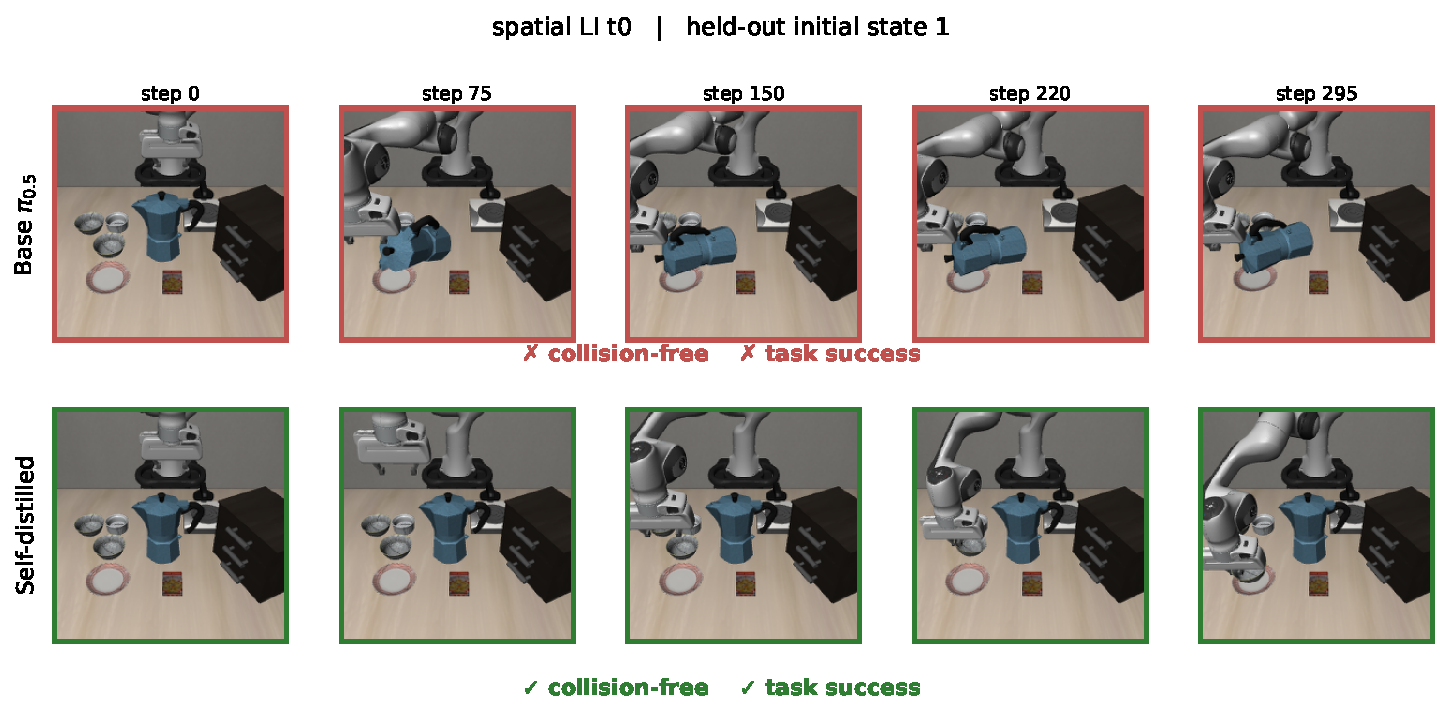
\includegraphics[width=\linewidth]{figures/fig_filmstrip.pdf}
%    \caption{...}
%    \label{fig:filmstrip}
%  \end{figure}
% =====================================================================================
\section{Does the Source of the Demonstrations Matter?}\label{sec:res:source}

An alternative is to distill from a stronger, purpose-built self-safe expert. This section explores this approach which works as an ablation to the previous one. A sampling-based motion planner was implemented as a privileged expert: RRT-Connect in joint space
with clearance inflation, followed by inverse kinematics and playback as operational-space deltas. It produced 318 successful demonstrations, across 18 of the 24 scenes.

\begin{table}[htbp]
\centering
\caption{Comparison of demonstration sources for policy distillation.}
\label{tab:demo_source_comparison}
\begin{tabular}{lcc}
\toprule
\textbf{Policy} & \textbf{TSR (95\% CI)} & \textbf{Collision rate (95\% CI)} \\
\midrule
Base, no shield                     & 58.3\% [49.4, 66.8] & 82.5\% [74.7, 88.3] \\
Planner-distilled, no shield        & 54.2\% [45.3, 62.8] & 80.0\% [72.0, 86.2] \\
Self-distilled (round 1), no shield & \textbf{82.5\% [74.7, 88.3]} & \textbf{19.2\% [13.1, 27.1]} \\
\bottomrule
\end{tabular}
\end{table}

The planner-distilled policy is statistically indistinguishable from the undistilled base policy on
both metrics and the only variable is the demonstration source (Section~\ref{sec:distillation}).

An interactive DAgger variant was also attempted and is reported in Appendix~\ref{app:dagger}; it did not alter the conclusion of the matched comparison below.

\paragraph{The planner is not a weaker teacher.}
It might be supposed that the planner's demonstrations simply contain less safety information.
They do not. Run unshielded on spatial task~0 the expert collides in 5 of 8 episodes, with
contact from arm links, gripper, held object and scene objects alike; run shielded it collides
in none. Its demonstrations depend on the shield to the same degree the policy's own do, and
both sets were collected under it. The demonstration sets are therefore matched in correction
signal, and differ in the states they occupy.


\paragraph{The mechanism is state coverage.}
Figure~\ref{fig:state_coverage} takes the base policy's own visited states and asks
how closely each demonstration set approaches them.

Subsampled to equal size per scene, the shielded rollouts cover 37.7\% of the policy's own
states within 2,cm against the planner's 22.8\%, and cover better in 15 of the 18 scenes
holding both demonstration types. Without that control the two sets are near-indistinguishable
at 37.7\% against 32.8\%, so the matching is load-bearing rather than cosmetic.

Figure~\ref{fig:state_coverage}(b) shows the shape of the difference. The planner is a
scripted controller and traces near-identical paths from a given initial condition, so its
demonstrations form tight deterministic bands; the states the policy actually visits are diffuse
and lie largely between and around them. The two distributions are not disjoint, but the planner's density is concentrated where the policy is not.

SAFE-GIL shows a foreign expert can teach safety once it is steered into the states a learner's
errors produce. The planner here was not built that way, so the comparison isolates the state
distribution rather than the teacher's identity. Whether a planner given that treatment would
transfer is untested (Section~\ref{sec:disc:future}).

Two limits apply. Coverage is measured on end-effector position, 3 of the 8 observed dimensions,
so it says nothing about joint configuration. And it is descriptive rather than causal: the
matched comparison establishes that the demonstration source mattered, while the coverage figure
proposes how the two sources differ.

\begin{figure}[htbp]
  \centering
  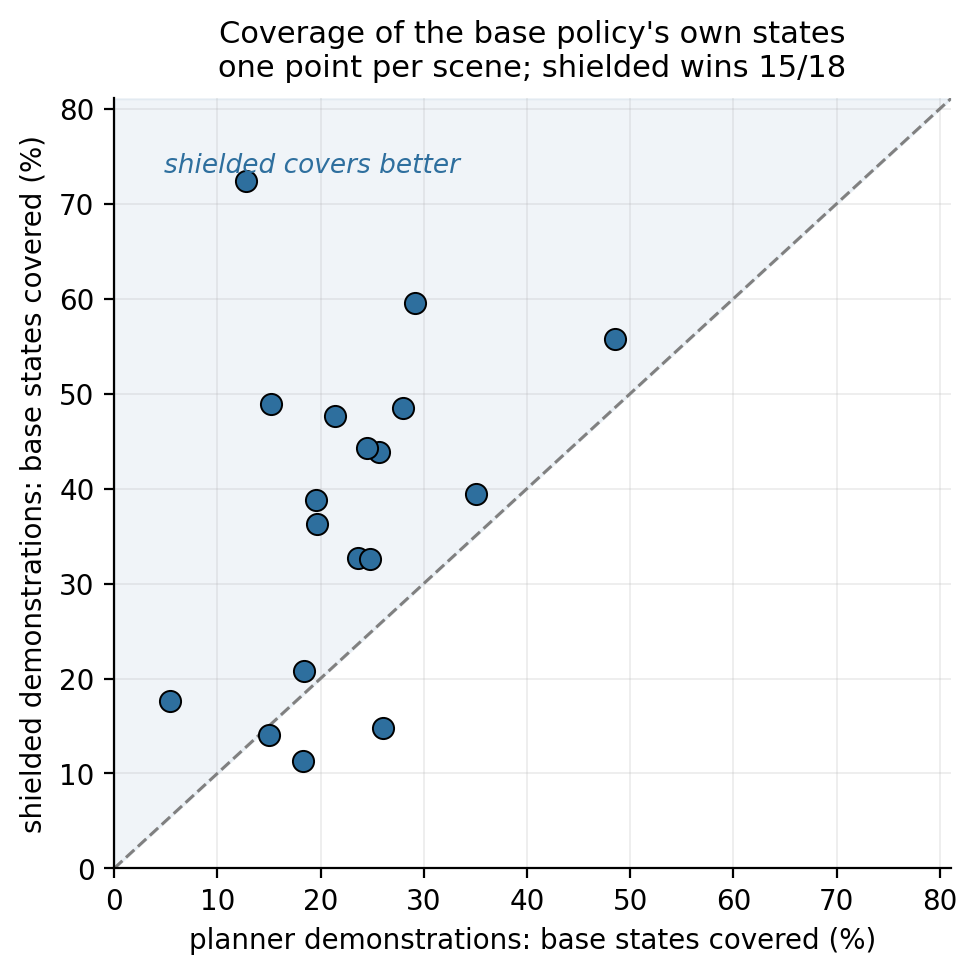
\includegraphics[width=\linewidth]{figures/fig_state_coverage.png}
  \caption[State coverage of the base policy's own trajectories]{%
    Both
    demonstration sets are subsampled to equal size per scene (30 resamples).
    \textbf{(a)} The shielded rollouts cover the policy's own states
    better in 15 of 18 scenes, 37.7\% against 22.8\% pooled.
    \textbf{(b)} The same comparison on the widest-gap scene. The planner's demonstrations
    form tight, near-deterministic trajectory bands, while the states the policy actually
    visits are diffuse and largely elsewhere.}
  \label{fig:state_coverage}
\end{figure}

\paragraph{Where the teacher had nothing to say.}
Six of the 24 scenes contain no planner demonstrations, so roughly 30 of the 120 evaluation
rollouts test whether the expert could solve the scene at all rather than whether distillation
worked. The gap is systematic rather than random --- the planner fails entirely on
elevated-target tasks, a kinematic limit of the controller rather than a collision-avoidance
one (Appendix~\ref{app:controller}). Restricting to the 18 scenes with training data does not
change the outcome, but both slices are worth distinguishing: the 24-scene figure conflates
scenes where the teacher had nothing to say with scenes where it spoke and was not understood.

\section{What Can the Shield Not Reach?}\label{sec:res:scope}

The shield reduces collisions to 13.3\% but not to zero. This section identifies what the residual
consists of, using per-body collision decomposition. 

\begin{table}[htbp]
\centering
\begin{threeparttable}
\caption[Residual collisions by culprit body]{%
  Per-body attribution of collisions in 120 episodes.}
\label{tab:culprits}
\begin{tabular}{lrrrrr}
\toprule
\textbf{Policy} & \textbf{Collided} & \textbf{Gripper} & \textbf{Arm link}
  & \textbf{Held object} \\
\midrule
Base, no shield        & 99 & 71          & 17 & 36 \\
Base + shield          & 16 & \textbf{0}  & 15 & \phantom{0}0 \\
\addlinespace[2pt]
Round 1, no shield     & 23 & \phantom{0}7 & 13 & \phantom{0}9 \\
Round 1 + shield       & 10 & \textbf{0}  & \phantom{0}8 & \phantom{0}1 \\
\addlinespace[2pt]
Round 2, no shield     & 21 & \phantom{0}8 & \phantom{0}8 & \phantom{0}7 \\
Round 2 + shield       & 11 & \textbf{0}  & \phantom{0}9 & \phantom{0}0 \\
\bottomrule
\end{tabular}
\end{threeparttable}
\end{table}

The split is the one Section~\ref{sec:barrier} predicts. Where the barrier's model is precise and
the constrained velocity is the commanded one --- the end-effector --- collisions are eliminated
outright: not one gripper contact across 360 shielded episodes, so the discrete-time
approximation of Section~\ref{sec:shield} holds in practice. Where the model is coarse and the
velocity is inferred, they persist: arm links account for 15 of the 16 residual collisions in the
shielded baseline.

This bears on how Section~\ref{sec:res:internalise} should be read. The distilled policy's
shield-free figure sits within a few points of what its teacher actually achieved, not of a
perfect one --- the teacher's ceiling is set by approximation error in the constraint rather than
by an absence of authority.

\paragraph{The student exceeds its teacher.}
Arm-link collisions fall from 17 to 8 between the base and twice-distilled policies, while the
shielded baseline --- with those same constraints active --- still records 15. The student is
therefore not merely reproducing the filter's corrections: in the channel where the barrier is
least able to enforce anything, it does better than the barrier does.

The likely route is the retention criterion rather than the correction signal. Demonstrations
were kept only if nothing at all was displaced, arm links included, so the dataset encodes
whole-body avoidance that no constraint row ever expressed. Safety reaches the policy through
two channels --- imitation of corrections where the filter has authority, and outcome selection
where it does not --- and only the second can carry behaviour the barrier cannot represent.

This is stated with less confidence than the gripper result: 17/120 against 8/120 is
14.2% [9.0, 21.5] versus 6.7% [3.4, 12.6], and those intervals overlap.


\section{What Explains the Improvement?}\label{sec:res:mechanism}

Section~\ref{sec:res:internalise} showed that distilling the shielded policy's own clean rollouts
makes it dramatically safer without the shield; however, it does not explain why this is so. The
demonstrations were filtered on three properties at once --- the shield fired, the episode
succeeded, and nothing was displaced --- and two mechanisms are conflated in the filter.

Under the first, \textbf{distillation}, the policy imitates the shield's avoidance corrections.
This is the claim of this work. Under the second, \textbf{selection}, the improvement comes from
training a policy on its own successful episodes, a known self-improvement effect requiring no
shield. If the second mechanism accounts for the result, the shield is incidental and the contribution is a
rediscovery of filtered behaviour cloning.

To disambiguate this, a matched control was run.

\subsection*{The matched control}

The matched control held every variable constant except for switching off the shield when collecting the demonstrations.


\begin{table}[htbp]
\centering
\caption{The matched control. Both distilled conditions use 85 demonstrations passing an identical
  filter; they differ only in whether the shield was active during collection. $n = 120$ held-out
  rollouts per row, Wilson 95\% intervals.}
\label{tab:matched_control}
\begin{tabular}{lccc}
\toprule
\textbf{Condition} & \textbf{Demos} & \textbf{TSR (95\% CI)} & \textbf{Collision (95\% CI)} \\
\midrule
Undistilled base & ---            & 58.3\% [49.4, 66.8] & 82.5\% [74.7, 88.3] \\
Control, shield \textbf{off}  & 85 & 50.0\% [41.2, 58.8] & 84.2\% [76.6, 89.6] \\
Matched, shield \textbf{on}   & 85 & \textbf{75.8\% [67.4, 82.6]} & \textbf{26.7\% [19.6, 35.2]} \\
\bottomrule
\end{tabular}
\end{table}

Compared to the base policy, the control has a marginally worse collision rate and more substantial TSR degradation. So, success-filtering by itself is unsuccessful in this benchmark. At the same demonstration count and under the same filter, the shielded condition reaches 26.7\%, with a confidence interval disjoint from the control's. Therefore, the difference between the two conditions is attributable to the shield. The activation rate corroborates this independently: after distillation the shield finds materially less to correct (Table~\ref{tab:internalisation}), and a policy that merely succeeded more often would not require \emph{less} safety intervention.

Nonetheless, the control run provided a relevant insight. Even though the collision total remained flat, per-body attribution shows arm-link collisions decrease from 17 to 6 while end-effector collisions remained high at 44. In line with Section~\ref{sec:res:scope}, selection therefore does transfer avoidance in the channel the barrier doesn't express, but its insufficient on its own. The 2 mechanisms are complementary rather than competing. The shield provides end-effector safety guarantes that distill, while selection improves overall safe behaviors for the rest of the robot arm components.

\paragraph{Observation aliasing, tested and rejected.}
Section~\ref{sec:res:source} showed that the planner's demonstrations did not transfer while the
policy's own shielded rollouts did. The intuitive explanation is that the shield's corrections
depend on state the policy cannot see: $\pi_{0.5}$ observes an image and eight proprioceptive
dimensions but no joint angles, and a 7-DoF arm can place the end-effector identically with the
elbow in very different positions --- so two training samples could look identical while carrying
contradictory targets, and behaviour cloning would average them. This was asserted early in the
project and never measured, though it is measurable from the demonstration files alone: for each
dataset, the disagreement between the target actions of observation-neighbours, normalised by the
disagreement between random pairs, compared at matched observation \emph{radius} rather than
matched neighbour count, since a nearest-neighbour ratio conflates aliasing with sampling density
and the planner's trajectories are far denser.

Figure~\ref{fig:aliasing} shows the prediction reversed. The planner's demonstrations are roughly
twice as \emph{well} determined by the observation at every radius: the teacher that fails to
distil has the cleaner observation-to-action mapping, and the teacher that succeeds is the more
aliased of the two. In hindsight the direction is unsurprising, since a scripted controller is
close to a deterministic function of state --- but the prediction was recorded before the planner
figure was computed, and aliasing is not the binding constraint. Distribution shift and
action-distribution mismatch remain as candidates.

\begin{figure}[htbp]
  \centering
  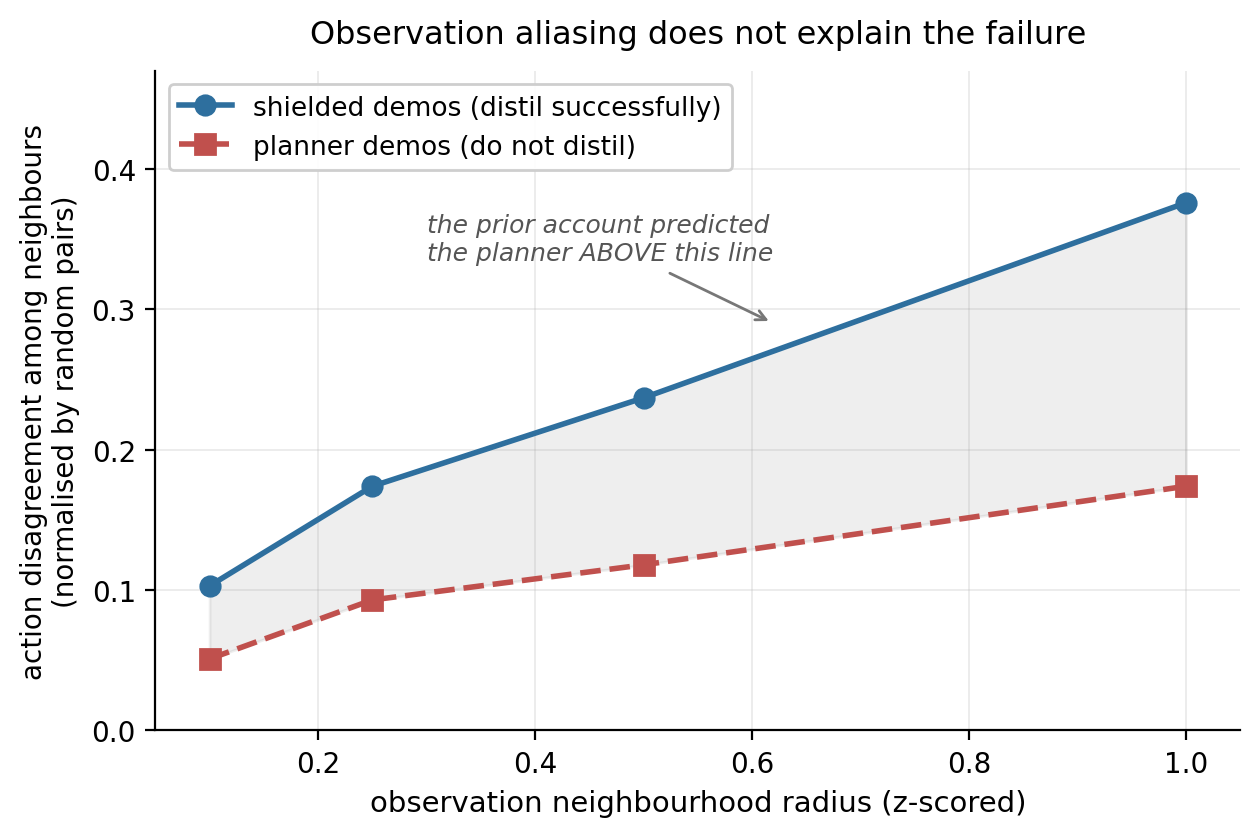
\includegraphics[width=0.72\linewidth]{figures/fig_aliasing.png}
  \caption[Observation aliasing does not explain the transfer failure]{%
    A prediction of this project, refuted by its own data. If the planner's corrections were
    poorly determined by what the policy observes, its curve would lie \emph{above} the shielded
    one. It lies consistently below, by a factor of roughly two at every radius.}
  \label{fig:aliasing}
\end{figure}


\section{Are There Other Channels for Safety?}\label{sec:res:channels}

Four further mechanisms were tested.
Table~\ref{tab:negatives} summarises them.

\begin{table}[htbp]
\centering
\begin{threeparttable}
\caption[Mechanisms tested and rejected]{%
  Mechanisms tested and rejected, with the scope at which each negative is claimed. None is a
  general claim about its method class.}
\label{tab:negatives}
\footnotesize
\begin{tabular}{p{0.17\linewidth}p{0.24\linewidth}p{0.22\linewidth}p{0.27\linewidth}}
\toprule
\textbf{Mechanism} & \textbf{What was tested} & \textbf{Outcome} & \textbf{Scope of the negative} \\
\midrule
Scalar-reward RL
  & Flow-SDE GRPO on the action head, 4 configurations $\times$ 6 rounds, one scene
  & Either collapses to inaction or learns nothing; no setting does both
  & The reward design and budget tested. Not safe RL as a class; constrained-MDP and
    world-model methods supply richer signals \\
\addlinespace[3pt]
Language-expressed constraint
  & One safety clause appended to the instruction, $n=60$ per condition, level II
  & No safety change; 23\% slower, 11.7 points less successful
  & The single phrasing tested: generic, unnamed referent, manner adverbial \\
\addlinespace[3pt]
Best-of-$N$ selection
  & $K \in \{4, 8\}$ candidates re-simulated per query, exact state rewind
  & No safe candidate on $\sim$60\% of queries; doubling $K$ buys 8.8 points
  & This policy and benchmark. The measurement it yields is reported as the result \\
\addlinespace[3pt]
Generative uncertainty as a runtime monitor
  & Three statistics of the stored flow-denoising chain, scored as AUC for predicting whether an
    episode collided
  & At chance for the base policy (0.461). The distilled policy inverts consistently
    (0.350, i.e.\ 0.65 flipped) but on 23 collision episodes
  & This policy and benchmark, and episode-level prediction. The inversion is roughly two standard
    errors from chance and is reported as suggestive \\
\bottomrule
\end{tabular}
\begin{tablenotes}[flushleft]\footnotesize
\item A further \emph{explanation}, as opposed to a mechanism, was also tested and rejected:
  observation aliasing does not account for the transfer boundary
  (Section~\ref{sec:res:mechanism}).
\end{tablenotes}
\end{threeparttable}
\end{table}


\subsection*{Scalar-reward reinforcement learning}

RL was tried first, and its failure motivated the imitation approach.

The setup was flow-SDE GRPO on $\pi_{0.5}$'s flow-matching action head: the deterministic sampling
ODE is converted to an equivalent SDE so that log-probabilities exist and a policy gradient can be
taken. A LoRA adapter on the action head received gradients with the backbone frozen, matching the
trainable surface used for distillation in Section~\ref{sec:res:internalise}, so the comparison
between the two learning signals is not confounded by capacity. Rollouts used the CPS sampler at
noise 0.7 with ten denoising steps and clipping 0.2, on one level-II scene, with $K = 8$ rollouts
per group over six rounds. The reward combined success, direct collision, CBF activation rate and
progress terms.

\begin{figure}[htbp]
  \centering
  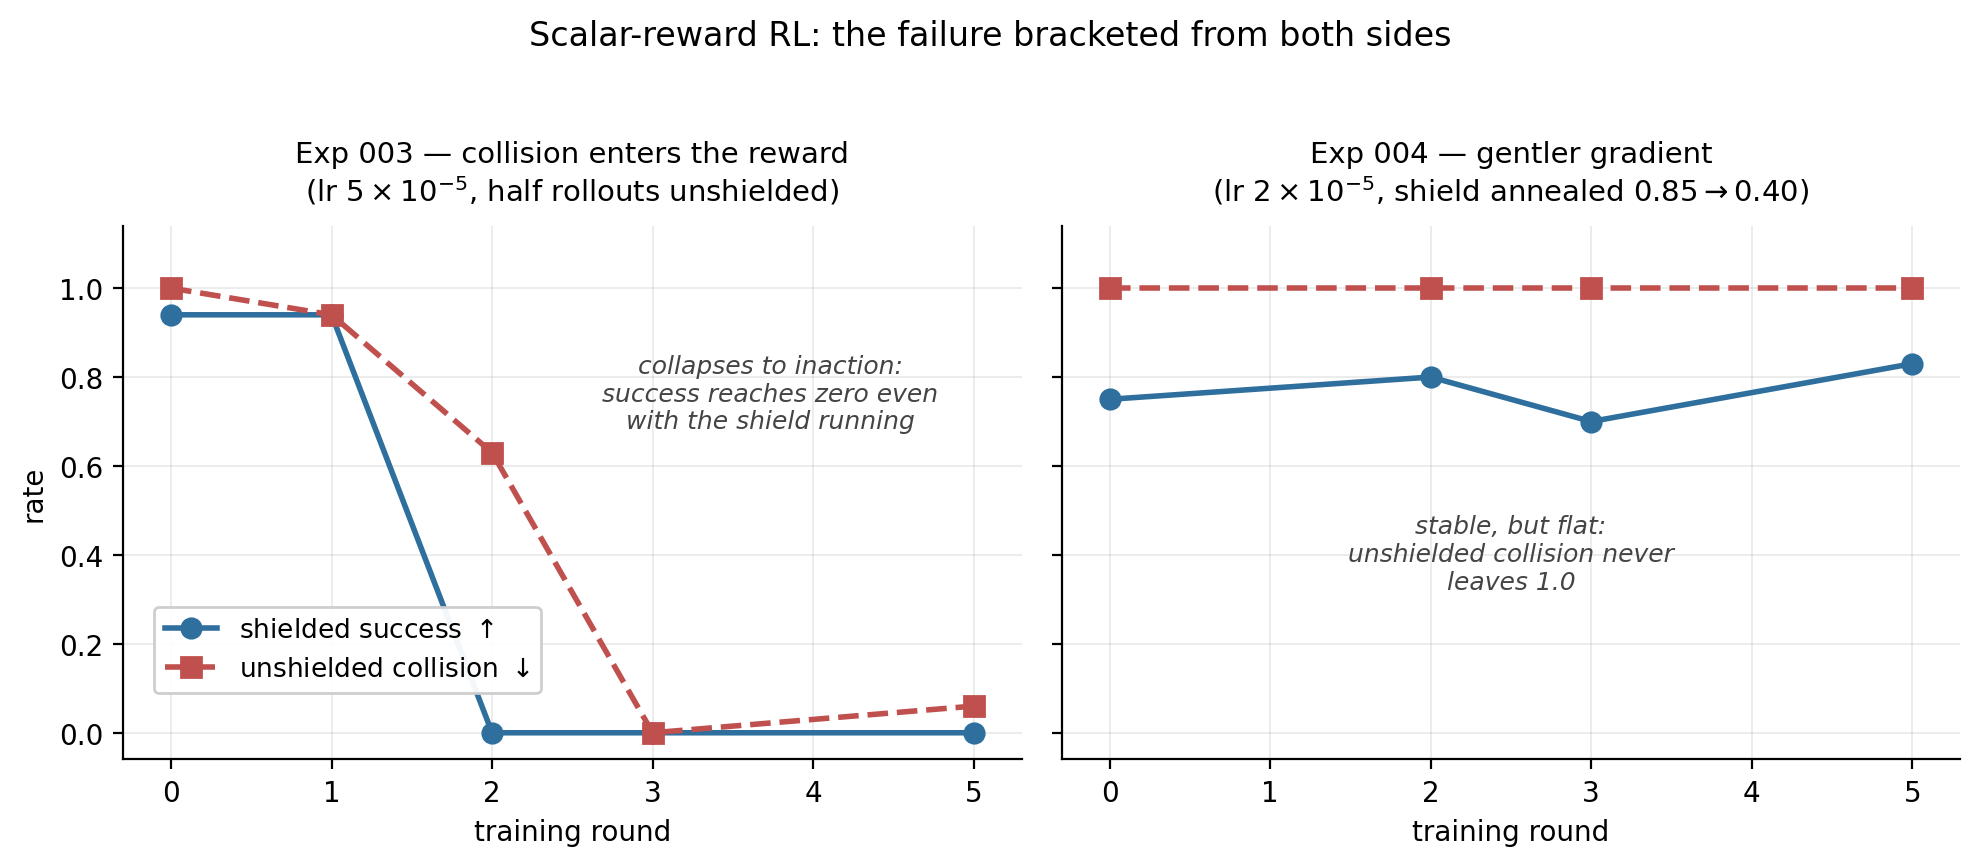
\includegraphics[width=\linewidth]{figures/fig_rl_bracket.png}
  \caption[Scalar-reward RL bracketed from both sides]{%
    The two informative configurations. \textbf{Left:} admitting real collisions to the reward
    moves the policy, and it collapses --- success reaches zero \emph{in the shielded condition
    too}, which the shield alone cannot cause, so the policy has found the trivial zero-collision
    optimum of doing nothing. \textbf{Right:} a lower learning rate with an annealed shield fixes
    the collapse and learns nothing, with unshielded collision pinned at 1.0 for six rounds.
    Neither panel alone is an argument; together they are the two sides of one knob.}
  \label{fig:rl_bracket}
\end{figure}

\paragraph{Too weak.}
With the shield active on every rollout, collisions never enter the reward directly --- the shield
prevents them --- so the only safety signal is the CBF activation penalty. Raising the learning
rate to $5 \times 10^{-5}$ and the activation weight to 1.5 left the policy flat.

\paragraph{Too strong.}
Running half of each group's rollouts unshielded puts real collisions into the reward, widening the
within-group spread to roughly $\Delta = 1.0$. The safety metric improved immediately and the task
collapsed with it. Two causes compound: the adapter diverged, since the mixed reward is far higher
variance than the flat one at the same learning rate; and the collision penalty punishes progress,
because in these scenes the obstacle lies between the gripper and the goal, so nearly all forward
motion collides early in training.

\paragraph{What the bracket establishes.}
The only configuration that moved the policy's behaviour collapsed it; every configuration stable
enough to preserve the task learned no avoidance. That is not a gap between two tuned settings but
the two sides of a single one. The learning signal and the destabilising signal are the same knob,
for two compounding reasons. A single scalar episode reward gives no per-step spatial credit, so
the policy cannot separate ``detour around the obstacle'' from ``stop moving toward the goal'' when
the obstacle lies on the path to the goal. And in a flow-matching policy, exploration \emph{is}
sampling noise, which is also what degrades the actions being evaluated.

This is precisely what the shield supplies and the reward does not. The barrier already computes
the correct action at every step it intervenes, in the same space the policy emits, so the credit
assignment the reward could not infer is simply given.

\subsection*{Safety expressed in language}

The experiment has the same checkpoint, seed, held-out initial states and
evaluation code for both conditions, differing only in a safety clause appended to the instruction. Twelve
level-II scenes at five initial states each give $n = 60$ per condition; level II was chosen
because of difficulty calibration.

\begin{quote}\small
\textbf{plain:} \texttt{pick up the black bowl between the plate and the ramekin and place it on
the plate}\\[3pt]
\textbf{safety:} \texttt{\dots{} and place it on the plate, being careful not to touch or knock
over any other objects}
\end{quote}

The phrasing is generic: it names no object, gives no spatial reference, and
states the constraint as a manner adverbial rather than a prohibition.

\begin{table}[htbp]
\centering
\caption{Effect of appending a safety clause to the instruction. $n = 60$ per condition, twelve
  level-II scenes, Wilson 95\% intervals.}
\label{tab:language}
\begin{tabular}{lccc}
\toprule
\textbf{Condition} & \textbf{TSR (95\% CI)} & \textbf{Collision (95\% CI)} & \textbf{ETS} \\
\midrule
Plain instruction       & 66.7\% [54.1, 77.3] & 70.0\% [57.5, 80.1] & 132.4 \\
Safety clause appended  & 55.0\% [42.5, 66.9] & 68.3\% [55.8, 78.7] & 162.4 \\
\bottomrule
\end{tabular}
\end{table}

The policy responds to the safety clause by marginally  decreasing collisions, succeeding less often, and taking longer to complete. 

The natural reading is that safety language elicits a general behavioural prior --- hesitancy,
reduced speed --- rather than a grounded avoidance behaviour. The model has learned that
safety-flavoured instructions correspond to cautious-looking motion, and that association is not
connected to the geometry of the scene.

ROAD-VLA got similar negative results from their text-based grounding experiments~\cite{wang2026roadvla}. They attribute the failure to a modality gap preventing discrete text from supplying the grounding continuous control requires.

\subsection*{Best-of-$N$ selection}

If safety varied across the actions a policy might sample from a given state, it could be obtained
by rejection: draw $K$ candidate action chunks, simulate each, execute the safest. The sampler must
be stochastic for candidates to differ, so the matched control is $K = 1$ at the same noise level
rather than the deterministic policy used elsewhere in this chapter. Making the measurement
trustworthy required the simulator to be rewound exactly between candidates; snapshot and restore
were verified to machine precision before any result was recorded.

\begin{figure}[htbp]
  \centering
  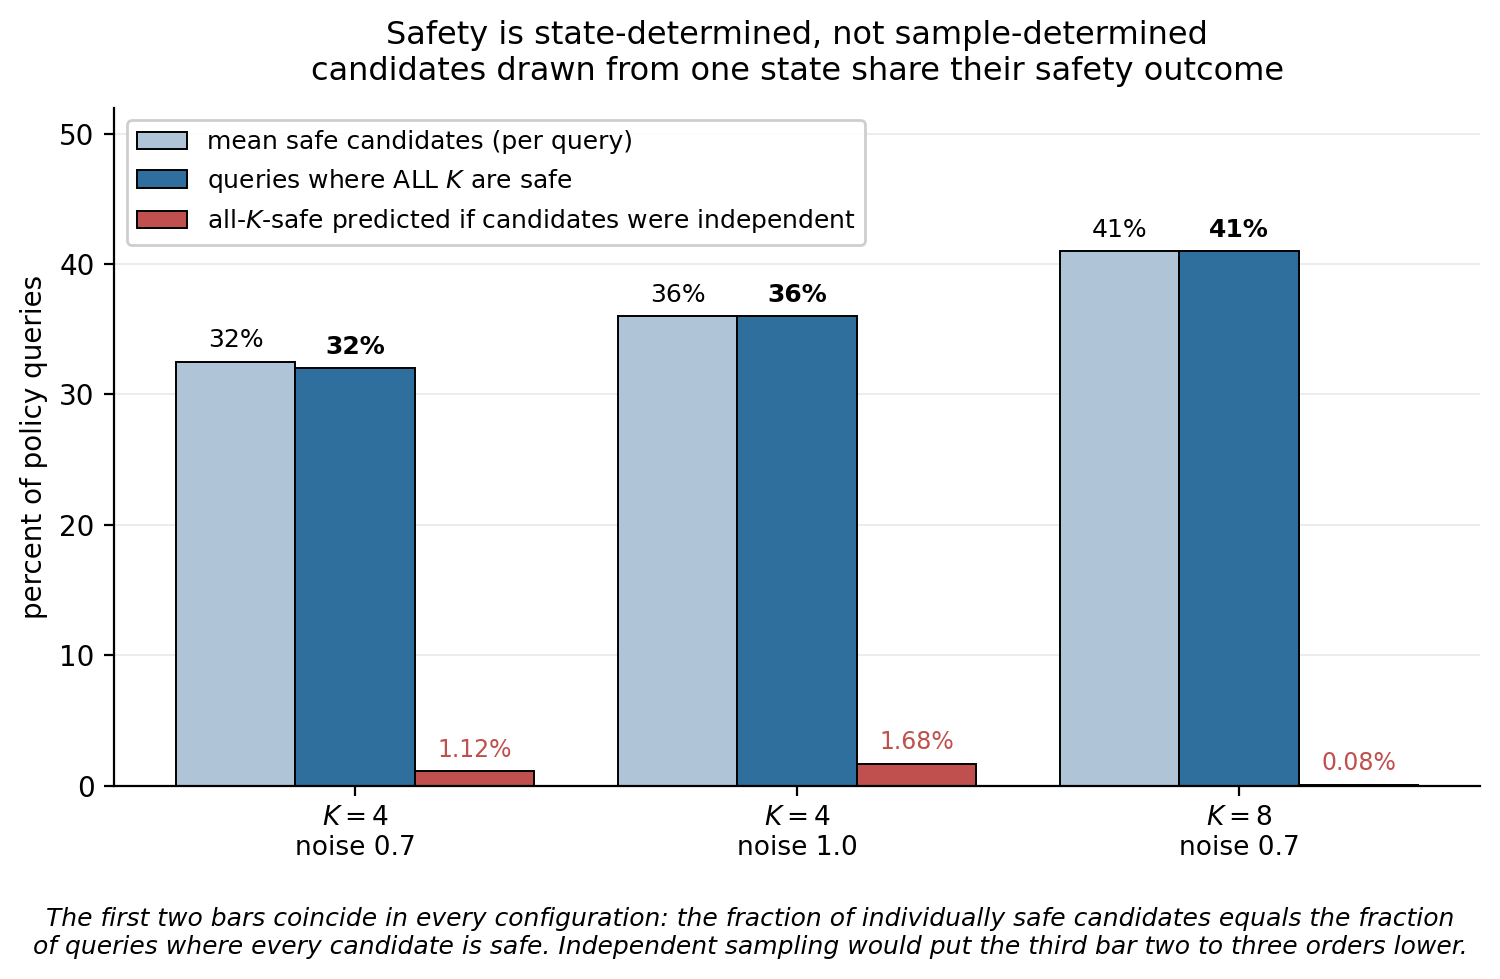
\includegraphics[width=0.82\linewidth]{figures/fig_bon_correlation.png}
  \caption[Within-state safety correlation in a VLA policy]{%
    Why rejection sampling cannot help here. In every configuration the fraction of individually
    safe candidates coincides with the fraction of queries in which \emph{all} $K$ are safe, so a
    query is $0$-of-$K$ or all-of-$K$ safe and almost never in between. Independent sampling would
    make the all-$K$-safe rate two to three orders of magnitude smaller (right-hand bars).}
  \label{fig:bon}
\end{figure}

As a method this is negative: on roughly 60\% of queries no candidate was safe, and buying more
candidates barely moved it --- doubling $K$ from four to eight recovered 8.8 percentage points for
twice the compute, and raising the noise recovered 3.7.

The measurement underneath it is the more interesting result. The mean safe fraction and the
all-$K$-safe fraction coincide in all three configurations. Were the candidates independent draws,
the all-$K$-safe rate would be $p^{K}$: 1.1\% at $K = 4$ and 0.08\% at $K = 8$, against observed
values of 32\% and 41\%. The policy's samples from a given state are therefore near-perfectly
correlated in their safety outcome.

Safety in this policy is consequently \textbf{state-determined rather than sample-determined}, at
least on this benchmark. Once a state is reached the outcome is largely fixed, and no amount of
choosing among actions recovers it --- the leverage lies in not reaching the state. This also
explains a result that would otherwise look inconsistent: episode-level filtering worked
(Section~\ref{sec:res:mechanism}) while action-level selection cannot, because episode-level
selection chooses between trajectories that reached \emph{different states}, which is the axis
along which variation actually exists.

The correlation measurement is offered here as the contribution rather than the selection method.
It is, as far as this work is aware, the first measurement of candidate-level safety correlation in
a VLA policy, and it is the sharpest available statement of the reachability
theme running through Sections~\ref{sec:res:scope}, \ref{sec:res:mechanism} and the discussion that
follows.

\subsection*{Generative uncertainty as a collision predictor.} Uncertainty was also tested as a barrier-free monitor: $\pi_{0.5}$ stores the full denoising chain
for every action, and if the policy were less certain where safe and unsafe behaviours are both
plausible, that chain would carry a risk signal requiring no obstacle geometry at all. It does
not --- the association is at chance for the base policy, and the distilled policy's consistent
\emph{inversion} suggests, on limited evidence, that its remaining failures are confident ones.

\chapter{Discussion}\label{ch:discussion}

\section{Why Imitation Succeeds Where Scalar-Reward RL Fails}\label{sec:disc:mechanism}

Both approaches attempted here aim at the same target --- move the policy toward the behaviour the
shield induces --- and differ only in the signal used. That difference turns out to be decisive,
and for a structural reason rather than a tuning one.

A scalar reward communicates the target through one number per trajectory, leaving the policy to
infer which of several hundred actions was responsible. In a flow-matching policy the only lever
available for that inference is sampling noise, so exploration and credit assignment are the same
knob: raising it enough to distinguish good actions from bad also degrades the actions being
evaluated. Section~\ref{sec:res:channels} brackets the consequence from both sides, and no working
point exists between them. Imitation removes the inference entirely. The shield does not report
that a trajectory was unsafe; it reports what should have been done instead, at each step where it
intervened, in the space the policy emits. Credit assignment is given rather than inferred.

That this is not trivial is established by a control in the literature rather than by argument.
Guerrier et al.\ train under an active CBF filter and then remove it, and their agent does not
internalise the constraint --- its critic assigns high value \emph{inside} the
obstacle~\cite{guerrier2025guardrails}. Their agent's actions were overridden while its objective
remained a scalar reward, so no gradient ever pointed toward the corrected action. Exposure to a
shield during training does not by itself transfer safety; the imitation objective is what does the
work, which disposes of the deflationary reading that any policy trained under a shield would end
up safe.

\subsection*{What the Boundary Result Shows}

Dense per-step supervision is necessary but not sufficient. The planner's targets were equally
dense and equally corrected, and transferred nothing. What separated the two teachers was where
their demonstrations sat: at matched sampling the planner covers the states the student reaches
substantially less well (Figure~\ref{fig:state_coverage}).

The operative variable is therefore the state distribution the supervision covers, not the identity
of the teacher --- a distinction the literature supports independently. SAFE-GIL clones an MPC or
PID expert and IntervenGen replays human corrections; both teachers are foreign to the learner, and
both transfer safety, because both take care that the demonstrations sit at states the learner's
errors would produce~\cite{ciftci2025safegil,hoque2024intervengen}. Self-distillation is one route
to that coverage rather than the only one. Its practical advantage is that it needs no disturbance
model or human operator: the policy visits its own failure states unprompted.


\section{The Cost of Internalised Caution}\label{sec:disc:cost}

% Mine
The main cost is in execution time. The distilled policy is roughly 14\% slower. It takes a more conservative route, and given the focus of this work in safety instead of performance, this is to be expected.

\begin{figure}[htbp]
  \centering
  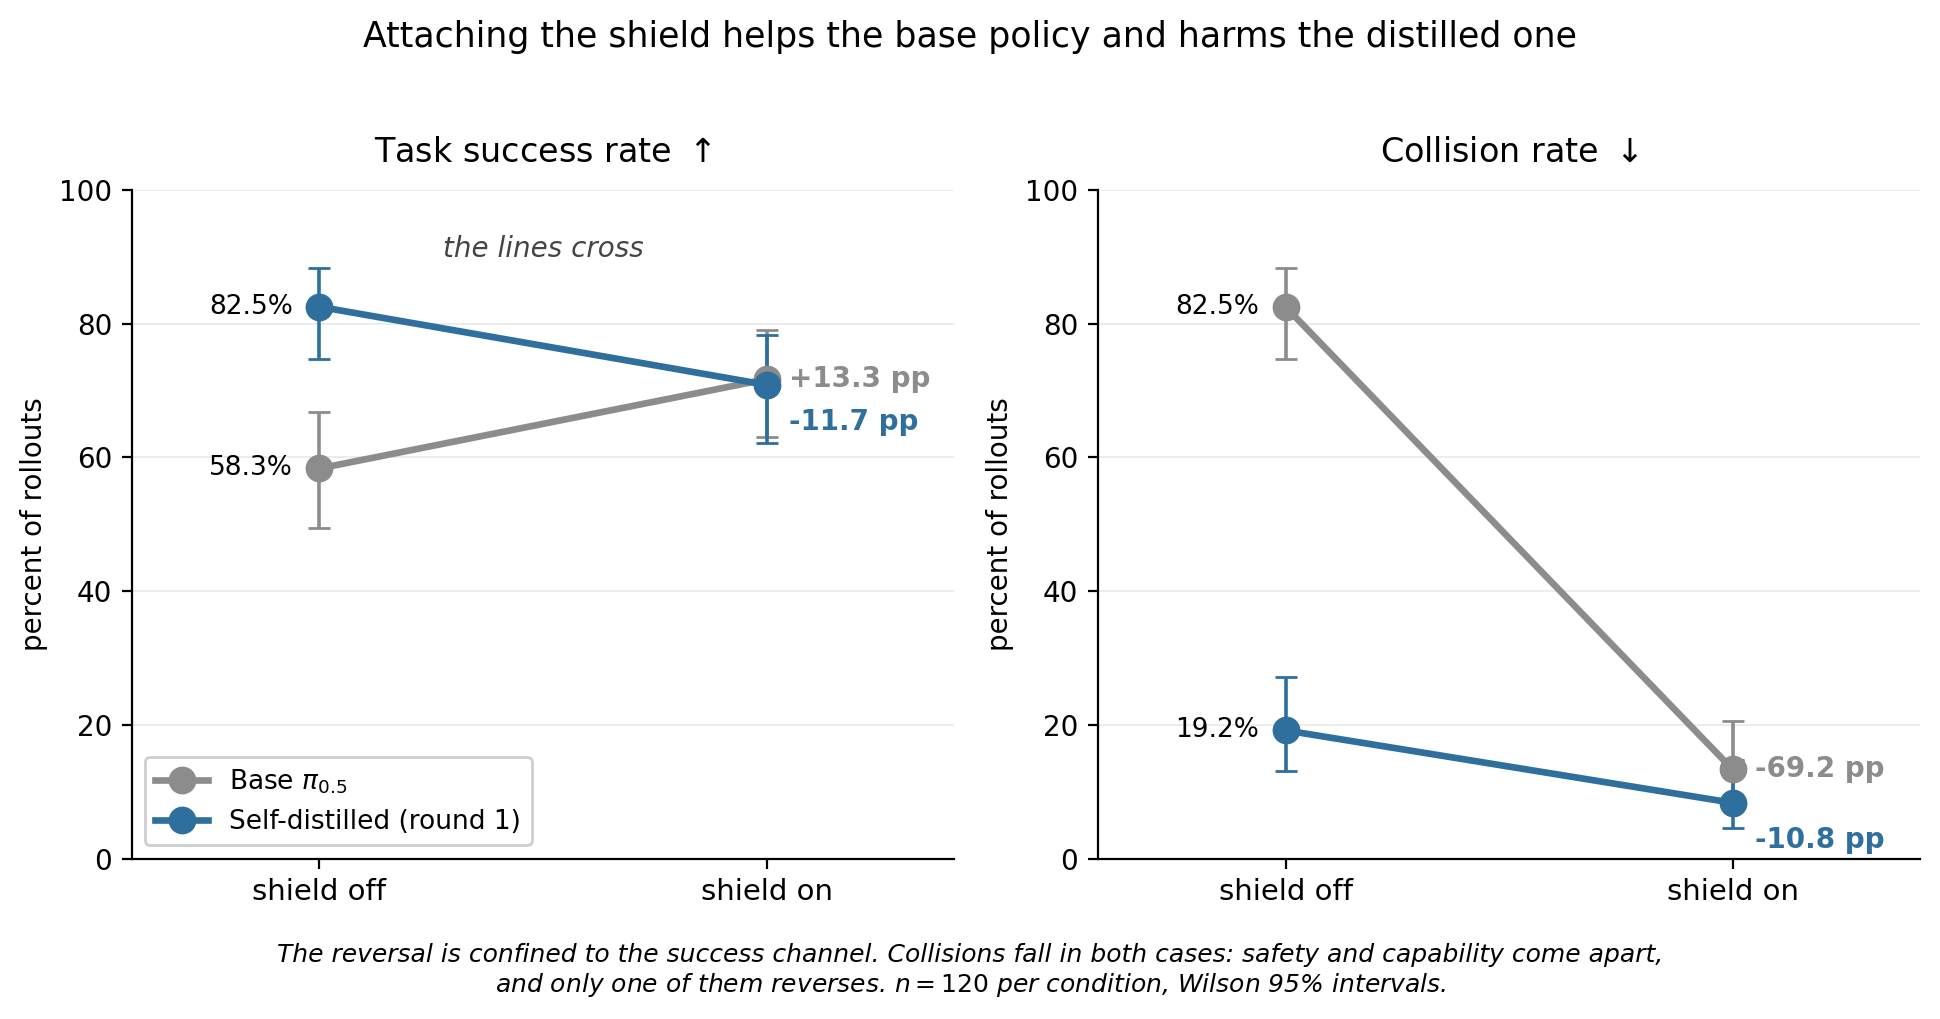
\includegraphics[width=\linewidth]{figures/fig_stacking.png}
  \caption[The cost of combining mechanisms]{%
  Attaching the shield raises the base policy's
    success and lowers the distilled policy's, but collisions fall in both cases.}
  \label{fig:stacking}
\end{figure}

There is a cost trade-off that comes from combining mechanisms rather than of distillation itself. As shown in Figure 5.1,  applying the shield to the distilled policy improves safety further but reduces success by similar amounts. When the distilled policy already avoids the obstacle, the shield's safe action projection perturbs actions that were already both safe and competent, leading to safety-induced distribution shift. This result is congruent to what is reported in VLSA, and reaffirms the relevance of self-distillation as an alternative approach to achieve safety while retaining competence.

A second distillation round neither improved nor
eroded performance, in contrast to an earlier DAgger-style experiment in this project that degraded
across rounds (Section~\ref{sec:res:source}). One round was sufficient, and iterating was not
harmful.

The trade runs both ways. Re-attaching the shield costs success but restores the online constraint
satisfaction a formal safety argument requires, and it produces the highest collision-avoidance
rate of any configuration tested --- 91.7%, at a success rate statistically indistinguishable
from shielding the base policy. Where a safety case demands a runtime constraint, distilling first
is therefore the better starting point. That the residual is 8.3% rather than zero is a reminder
that the guarantee is continuous-time and the implementation approximates it
(Section~\ref{sec:barrier}).

\section{Limitations}\label{sec:disc:limitations}

\paragraph{Simulation only.}
Every result is from SafeLIBERO. No physical robot was used and no claim of sim-to-real transfer is
made.

\paragraph{No formal guarantee is inherited.}
The conditions under which a learned
controller inherits input-to-state safety instead~\cite{cosner2022il_cbf} are set out in
Section~\ref{sec:bg:learned}, and none holds here: the shield is a nominal rather than a robust
QP, the plant is not a known control-affine system, and neither a bounded learning error nor a
Lipschitz constant is available for a 3-billion-parameter flow-matching policy. What is
demonstrated is an empirical reduction in collisions.

\paragraph{Privileged geometry.}
The barrier is constructed from obstacle poses and meshes read directly from the simulator. A
deployed system would estimate that geometry from perception and inherit the resulting error, so
every shielded figure reported here is an upper bound for this class of filter. The distilled
policy uses no geometry at inference, but the
dependency remains during \emph{training}.

\paragraph{Approximate robot model.}
The barrier represents the robot with spheres rather than its exact shape, because the exact
version would not solve fast enough to run at every control step (Section~\ref{sec:barrier}).
Section~\ref{sec:res:scope} argues the remaining collisions happen where those spheres fit worst.
That is a plausible reading of which bodies collided, but how accurate the constraint actually
was is never measured directly.

\paragraph{Single training seed.}
Each distilled policy is one training run and seed variance is unquantified.

\paragraph{Single policy and action space.}
Everything here uses one model, $\pi_{0.5}$, which produces chunks of actions by integrating a
flow field. Two results depend on that design --- the reinforcement-learning negative and the
best-of-$N$ measurement --- and may not carry over to policies that emit one action at a time.

\paragraph{Scope of the negative results.}
The reinforcement-learning result is a finding about the reward design and budget tested, not
about safe reinforcement learning as a class. Constrained-MDP~\cite{safevla} and
world-model~\cite{safedojo} approaches supply materially richer constraint signals --- the latter
on this same benchmark --- but both require substantially more compute than was available here:
large-scale constrained online interaction in one case, and training an action-conditioned video
world model in the other. Flow-SDE GRPO was chosen as the variant that could be run at this
scale, and the negative should be read accordingly. Similarly, the best-of-$N$ measurement
supports a state-dominant account of collision risk in this policy and benchmark rather than a
general claim about generative policies.

\paragraph{Attribution caveats.}
The per-body attribution is a documented lower bound that can miss delayed or indirect contacts.

\section{Future Work}\label{sec:disc:future}

\textbf{A physical robot} is the most direct extension. Whether internalised avoidance survives contact
dynamics, calibration error and a real perception pipeline is the question this work most needs
answered, and Section~\ref{sec:disc:cost} suggests the deployment configuration to test: the
distilled policy with the shield reattached, which reached the highest collision-avoidance rate of
any arm evaluated while keeping the runtime constraint a safety case would require.

\textbf{Repeating the training across seeds} is the cheapest outstanding item and addresses the
weakest one. Each distilled policy here is a single run, so the training variance behind the
headline is unquantified even though the evaluation variance is not.

\textbf{Perception-grounded barriers} would remove the privileged-geometry dependency and measure
how much of the reported safety survives estimation error --- the same question a physical
deployment asks, isolated from the rest of the reality gap. Learned safety representations offer
one route~\cite{meng2024conbat,sun2025lpb}, though both retain the inference-time correction this
work removes.

\textbf{A whole-body barrier} with proper link geometry and directly constrained link velocities
would lower the shield's own floor (Section~\ref{sec:res:scope}); whether that improvement then
distils is separately testable. It would also make CBF-guided sampling worth testing, since the
existing implementation was verified against a closed-form projection but wired to an
end-effector barrier, and so never activated on the scenes where arm links collided.

\textbf{Other architectures and moving obstacles} bound the generality of the result. The
best-of-$N$ and reinforcement-learning findings depend on chunked flow sampling and may not hold for
policies emitting single actions, and every scene here is static --- the case that matters for
deployment is a constraint that moves.

Finally, \textbf{separating the surviving explanations} would say something general about when
demonstrations transfer between controllers. Observation aliasing was measured and rejected
(Section~\ref{sec:res:mechanism}) and state coverage is supported but measured only on
end-effector position; distribution shift and action-distribution mismatch remain. A direct
comparison against model-based safe RL on this benchmark~\cite{safedojo} would place distillation
against the strongest current alternative.



% ============================================================================
\chapter{Conclusion}\label{ch:conclusion}
\label{sec:conc}

This thesis asked whether the safety of an inference-time control-barrier
function shield can be distilled into a VLA policy. Under the specific conditions tested in this work, the answer is yes. Self-distilling $\pi_{0.5}$ reduced collisions from 82.5\% to 19.2\% \textbf{without running the shield at inference}, while increasing task success from 58.3\% to 82.5\% on held-out initial states. The resulting
policy achieved a collision-avoidance rate of 80.8\%, approaching the shielded policy's 86.7\%, and
one distillation round was sufficient.

Distillation therefore creates a choice between two operating points, and both improve on what was
available before. Run shield-free, the policy is safer and more capable than the model it came
from --- but the online constraint satisfaction that establishes forward invariance is
gone~\cite{ames2017cbf}, and what remains is an empirical reduction rather than a guarantee.
Reattached, the shield restores that constraint and yields the safest configuration measured:
8.3\% collisions at 70.8\% success, against 13.3\% and 71.7\% for the same shield on the
undistilled policy. Where a safety case demands a runtime constraint, distilling first therefore
costs nothing in success and lowers what the constraint is left to catch; and against the original
unshielded policy the same configuration is both more successful and an order of magnitude safer.
That the residual is 8.3\% rather than zero reflects the approximations of
Section~\ref{sec:barrier}, not the absence of the argument.

\section*{The Boundary Condition}

The transfer is bounded, and the bound is the more useful half of the result. A geometry-privileged
motion planner supplying dense per-step corrections produced no measurable improvement under a
matched comparison; filtering only for successful episodes produced none either. What separates the
teacher that worked from the one that did not is where its demonstrations sit. Transferable
supervision must correct the learner at states the learner itself reaches.

This is narrower than the claim it is easily mistaken for. Foreign teachers can transfer safety:
SAFE-GIL clones an MPC or PID controller and IntervenGen replays human
corrections~\cite{ciftci2025safegil,hoque2024intervengen}, and both succeed because both take care
that their demonstrations sit where the learner's errors would put it. The planner tested here
received no such treatment. Policy-proximal self-distillation predicts precisely this
outcome~\cite{wang2026roadvla}, but every teacher that work rejects is textual and every teacher it
accepts is derived from the student, so no foreign low-level controller appears anywhere in it.
Supplying one, and measuring what follows, is this thesis's contribution.

Two features of the result are not anticipated by that literature. Safety and task success improved
\emph{together}, where the closest prior method reports a tradeoff between them. And no disturbance
model was required: the shield corrects at states the policy reaches unprompted, where an
adversarial construction must manufacture them.

\section*{What Bounds the Claim}

The distilled student avoided arm-link collisions more effectively than the shield that supervised
it --- 8 against 15 --- which suggests trajectory imitation alone does not describe what was
learned. The Wilson intervals overlap, so the effect is suggestive rather than established
(Section~\ref{sec:res:scope}).

Three alternative mechanisms were tested and none substituted for shielded imitation, but each
negative is scoped rather than general. The reinforcement-learning result concerns the reward
design and budget tested, not safe reinforcement learning as a class: neither
constrained-MDP~\cite{safevla} nor model-based world-model approaches~\cite{safedojo} are
scalar-reward methods, and both require compute beyond what was available here. Language-specified
safety was tested at a single phrasing. And best-of-$N$ supports a state-dominant account of
collision risk \textbf{in this policy and benchmark} rather than a general claim about generative
policies.

\section*{What Is New, Stated Precisely}

Two neighbouring claims would be false and are not made. Learning safety from CBF-related
supervision is not new; it has been treated theoretically~\cite{cosner2022il_cbf}, and learning
from CBF demonstrations in simulation predates that work. Distilling a corrective signal into a
vision-language-action policy is not new either~\cite{wang2026roadvla}.

What is new is the conjunction: a control-theoretic safety filter, distilled from a VLA's own
shielded rollouts and evaluated with the filter \emph{removed}, in the setting where runtime
shielding is the current state of the art. With it comes the boundary condition --- a
geometry-privileged planner supplying dense low-level corrections does not transfer under a matched
comparison --- and one measurement rather than a method: within a given state, the safety outcomes
of a VLA's sampled action candidates are near-perfectly correlated, which is why action-level
rejection sampling cannot help where episode-level selection can
(Section~\ref{sec:res:channels}).

The practical conclusion is narrower than ``safety can be learned''. A runtime filter teaches a
policy the regularities it observes and corrects, and those corrections amortise into weights
without the per-step optimisation comparable learned-barrier methods retain at
inference~\cite{meng2024conbat,sun2025lpb}, and at a fraction of their training cost. But the
learned policy is only as broad as the states, hazards and geometry those corrections represent.
Runtime shielding remains necessary outside that envelope. Distillation reduces dependence on the
shield; it does not remove the need for a safety case.



% ============================================================================
\bibliographystyle{plainnat}
\bibliography{references}

\appendix
\chapter{Additional results}
% Per-suite and per-task breakdowns that would clutter the main text.

\paragraph{Interactive distillation, and the diagnostic that located its failure.}
Before the offline comparison reported above, the classical expert was distilled interactively in
the DAgger manner: the student drives, the expert labels the states the student visits, and the
aggregated dataset is retrained. This is the textbook remedy for exactly the coverage problem
identified below, and it made matters worse. Collision rose monotonically across rounds, from 44\%
to 75\%, with success pinned near zero.

The cause was not the coverage principle but a violated precondition. DAgger's correctness argument
requires a Markov oracle $\pi^{*}(s)$: the expert's label must be a function of the state it is
shown. The classical expert was implemented as a latched phase machine carrying hidden internal
state, so when the student drove erratically the expert's phase desynchronised from the observation
and the same image received contradictory labels across rounds. Behaviour cloning averaged them.

Isolating this required ruling out the alternative, that the imitation machinery itself was broken.
Hard-overfitting behaviour cloning on a single clean demonstration and evaluating on that same
episode returned success $1.0$ with zero collisions, establishing that normalisation, the
observation pipeline and adapter capacity were all sound, and that the fault lay in the labels. The
expert was then rewritten as a stateless reactive oracle, inferring its phase from observables at
every call~--- grasp from the measured gripper finger separation, transport from end-effector
height~--- and validated against the original on the same episodes, where it produced identical
outcomes episode-for-episode.

The rewrite made the expert Markov, and distillation still failed. That is what moved the
investigation from the interactive protocol to the teacher itself, and ultimately to the matched
offline comparison reported above. It is recorded here because the negative is easy to misattribute:
an interactive method failing against a non-Markov expert is a statement about the expert, not about
DAgger or about coverage.

\chapter{The Classical Controller Characterised on Its Own}\label{app:controller}

Section~\ref{sec:res:source} reports that six of the 24 scenes contain no planner demonstrations
and that the gap is systematic. This appendix gives the evidence, from the full-grid collection of
24 scenes $\times$ 36 attempts $=$ 864 rollouts under ground-truth geometry. A demonstration is
\emph{clean} if it succeeded and displaced no obstacle; the overall yield is 318/864, or 37\%.

\section{The Yield Is Bimodal, Not Uniformly Mediocre}

\begin{table}[htbp]
\centering
\caption{Clean demonstrations per scene, out of 36 attempts. Two scenes exceed 94\%; six produce
  nothing at all, so the aggregate of 37\% misrepresents both ends of the distribution.}
\label{tab:planner_yield}
\footnotesize
\begin{tabular}{lrlr}
\toprule
\textbf{Scene} & \textbf{Clean} & \textbf{Scene} & \textbf{Clean} \\
\midrule
object\_LI\_t3    & 35 (97\%) & spatial\_LI\_t2   & 17 (47\%) \\
object\_LII\_t1   & 34 (94\%) & spatial\_LI\_t1   & 14 (39\%) \\
goal\_LI\_t0      & 26 (72\%) & object\_LII\_t0   & 14 (39\%) \\
goal\_LI\_t1      & 26 (72\%) & spatial\_LII\_t2  & 14 (39\%) \\
goal\_LI\_t2      & 22 (61\%) & spatial\_LI\_t0   & 12 (33\%) \\
spatial\_LII\_t3  & 20 (56\%) & object\_LII\_t2   & 12 (33\%) \\
object\_LII\_t3   & 19 (53\%) & spatial\_LI\_t3   & 11 (31\%) \\
goal\_LII\_t2     & 17 (47\%) & goal\_LII\_t0     & \phantom{0}9 (25\%) \\
                  &           & object\_LI\_t0    & \phantom{0}8 (22\%) \\
                  &           & goal\_LII\_t3     & \phantom{0}8 (22\%) \\
\midrule
\multicolumn{4}{l}{\emph{Zero yield:} goal\_LII\_t1, goal\_LI\_t3, object\_LI\_t1,
  object\_LI\_t2, spatial\_LII\_t0, spatial\_LII\_t1} \\
\bottomrule
\end{tabular}
\end{table}

The failure is not a difficulty effect. Three of the six zero-yield scenes are level~I, while
spatial\_LII\_t3 reaches 56\% and object\_LII\_t1 reaches 94\%. Competence is task-specific rather
than level-specific, which rules out ``level~II is simply harder'' as the explanation.

\section{Three Separable Failure Mechanisms}

Phase occupancy from the per-step logs of the six zero-yield scenes separates three causes rather
than one. Counts measure time spent in a phase rather than terminal outcome.

\begin{table}[htbp]
\centering
\caption{Dominant execution phases in the six zero-yield scenes, with the two highest-yield scenes
  for contrast. Reaching \textsc{place} is what distinguishes success.}
\label{tab:planner_phases}
\footnotesize
\begin{tabular}{lll}
\toprule
\textbf{Scene} & \textbf{Dominant phases} & \textbf{Mechanism} \\
\midrule
goal\_LII\_t1     & \textsc{plan\_failed} 3150 (no other phase reached) & planning infeasibility \\
goal\_LI\_t3      & \textsc{done} 1553, \textsc{transport} 394          & task inexpressibility \\
object\_LI\_t1    & \textsc{approach} 1509, \textsc{transport} 714 (no \textsc{place}) & execution \\
object\_LI\_t2    & \textsc{approach} 1228, \textsc{transport} 1022, \textsc{place} 22 & execution \\
spatial\_LII\_t0  & \textsc{approach} 1437, \textsc{done} 545           & execution \\
spatial\_LII\_t1  & \textsc{done} 1214, \textsc{approach} 495           & execution \\
\midrule
object\_LI\_t3    & \textsc{approach} 413, \textsc{transport} 296, \textsc{place} 65 & --- \\
object\_LII\_t1   & \textsc{transport} 673, \textsc{approach} 420, \textsc{place} 78 & --- \\
\bottomrule
\end{tabular}
\end{table}

\paragraph{Planning infeasibility.}
In goal\_LII\_t1, \textsc{plan\_failed} is the only phase ever reached: RRT together with the
inverse-kinematics and clearance ladder never returns a collision-free plan, and execution is never
attempted. This is purely geometric.

\paragraph{Task inexpressibility.}
In goal\_LI\_t3 the plan executes to completion and the task is still not satisfied. The task is
\emph{open the top drawer and put the bowl inside} --- two-stage manipulation that a pick-and-place
waypoint sequence cannot represent. Zero yield here is a statement about what was implemented, not
about the method.

\paragraph{Execution and tracking failure.}
In the remaining four scenes a plan exists but the arm does not track it to placement: time
concentrates in \textsc{approach} and \textsc{transport} while \textsc{place} is barely or never
reached. The two highest-yield scenes are distinguished precisely by reaching \textsc{place}.

\section{Seven Iterations, and Why the Residual Is Structural}

\begin{table}[htbp]
\centering
\caption{Controller iterations, each with a measured diagnosis rather than a guess. The aggregate
  never leaves the 35--40\% band.}
\label{tab:planner_iterations}
\begin{tabular}{llr}
\toprule
\textbf{Version} & \textbf{Change} & \textbf{Clean ($n=48$)} \\
\midrule
v2  & clearance inflation                            & 40\% \\
v3  & clearance ladder + IK retry                    & 35\% \\
v4  & fallbacks                                      & 29\% \\
v5  & payload speed limit (object slipping from grip) & 38\% \\
v6  & scene settling before measurement              & 38\% \\
v8  & four fixes from visual inspection              & 35\% \\
v10 & orientation gate on waypoint arrival           & \textbf{40\%} \\
\bottomrule
\end{tabular}
\end{table}

Individual fixes are real and diagnosed --- the orientation gate took a closing error from
35.5\textdegree{} to 0.0\textdegree{} on a scene that had regressed to zero --- but each trades
scenes against one another rather than lifting the total. That pattern, across seven attempts, is
the evidence that the residual is structural rather than a tuning deficit.

\section{A Physical Constraint Mistaken for a Control Failure}

One earlier failure is worth recording for how it was diagnosed. Several bowl tasks sat at 0\%
success with the end-effector stalling roughly 5\,cm above the object centre, which reads as a
controller or inverse-kinematics problem. It was neither: the akita bowl is 11\,cm wide and the
gripper opens to 8\,cm, so a top-down straddle grasp is physically impossible and no controller
could have solved it.

The fix was a change of grasp strategy rather than of control. The gripper's fingers close along
the world $y$ axis, so offsetting the grip point by 5\,cm along that axis drops one finger inside
the bowl and one outside, pinching the rim on close. Bowls are selected for this mode by name while
cartons retain the top-down grasp, and the full three-dimensional grasp offset is tracked so that
placement drives the \emph{object} to the goal rather than the offset end-effector. A speed-capped,
$xy$-locked descent removes operational-space coupling drift. The spatial suite went from 0\% to
69\% with zero collisions.

This bears on how Section~\ref{sec:res:source} should be read. The teacher's remaining failures were
investigated for this class of explanation --- a physical constraint masquerading as a control
deficit --- and the elevated-target failures survived that check, which is what makes the
kinematic-limit reading credible rather than merely convenient.

\section{What This Does and Does Not Explain}

With full privileged geometry the controller reaches 37\% clean demonstrations, bimodally
distributed, failing through three separable mechanisms of which one is outside the scope of what
was built and one is purely geometric. A task-and-motion planner with drawer primitives would
address task inexpressibility; it would not obviously address execution failure, where most of the
lost yield sits.

Neither would change the distillation result. Section~\ref{sec:res:source} shows the planner
student is statistically indistinguishable from the undistilled base policy even when restricted to
the 18 scenes where demonstrations exist, so the outcome does not turn on the teacher's yield. What
separates the two teachers is the state distribution their demonstrations occupy, not the number of
scenes either could solve.


\chapter{Implementation notes}
% Reproduction commands. NOTE: the module guidance requires crediting AI tools
% used for code or writing, both in the codebase README and here. Be specific
% about which parts.

\end{document}
